% =========================================================================
% SENDA — guía educativa (edición pública del repositorio LATTIMEX, 2026-09-30)
% SPDX-License-Identifier: CC-BY-4.0
% Compilación: pdflatex guia_senda && bibtex guia_senda
% Después: pdflatex guia_senda (dos veces para resolver referencias).
% Datos y macros de las figuras incluidos en datos/; figuras en figuras/.
% =========================================================================
\documentclass[11pt,a4paper]{article}

\usepackage[T1]{fontenc}
\usepackage{lmodern}
\usepackage[spanish,es-noshorthands,es-nodecimaldot,es-tabla]{babel}
\usepackage[margin=2.4cm]{geometry}
\usepackage{microtype}
\usepackage{amsmath,amssymb}
\usepackage{booktabs}
\usepackage{array}
\usepackage{graphicx}
\usepackage{float}
\usepackage[font=small,labelfont=bf]{caption}
\usepackage{enumitem}
\usepackage[dvipsnames]{xcolor}
\usepackage{tikz}
\usetikzlibrary{arrows.meta,positioning,decorations.pathreplacing,calc,shapes.geometric}
\usepackage{pgfplots}
\pgfplotsset{compat=1.18}
\usepackage[most]{tcolorbox}
\usepackage{algorithm}
\usepackage{algpseudocode}
\usepackage{url}
\usepackage[colorlinks=true,linkcolor=MidnightBlue,citecolor=OliveGreen,urlcolor=MidnightBlue]{hyperref}

\floatname{algorithm}{Algoritmo}
\algrenewcommand\algorithmicrequire{\textbf{Entrada:}}
\algrenewcommand\algorithmicensure{\textbf{Salida:}}
\algrenewcommand\algorithmicwhile{\textbf{mientras}}
\algrenewcommand\algorithmicdo{\textbf{hacer}}
\algrenewcommand\algorithmicif{\textbf{si}}
\algrenewcommand\algorithmicthen{\textbf{entonces}}
\algrenewcommand\algorithmicelse{\textbf{si no}}
\algrenewcommand\algorithmicfor{\textbf{para}}
\algrenewcommand\algorithmicend{\textbf{fin}}
\algrenewcommand\algorithmicreturn{\textbf{devolver}}
\algrenewtext{ElsIf}[1]{\textbf{si no, si} #1 \algorithmicthen}
\algrenewtext{EndWhile}{\textbf{fin mientras}}
\algrenewtext{EndIf}{\textbf{fin si}}
\algrenewtext{EndFor}{\textbf{fin para}}
\newcommand{\SiDevolver}[2]{\State \textbf{si} #1 \textbf{entonces devolver} #2}

% --- Cajas didácticas ----------------------------------------------------
\definecolor{sendaink}{RGB}{19,34,31}
\definecolor{sendared}{RGB}{210,75,50}
\definecolor{sendagreen}{RGB}{11,131,96}
\newtcolorbox{ideaclave}[1][]{enhanced,breakable,colback=sendagreen!6,colframe=sendagreen!70!black,
  fonttitle=\bfseries,title={Idea clave#1},left=6pt,right=6pt,top=4pt,bottom=4pt}
\newtcolorbox{ejemplo}[1][]{enhanced,breakable,colback=MidnightBlue!4,colframe=MidnightBlue!70,
  fonttitle=\bfseries,title={Ejemplo resuelto#1},left=6pt,right=6pt,top=4pt,bottom=4pt}
\newtcolorbox{leccion}[1][]{enhanced,breakable,colback=sendared!6,colframe=sendared!85!black,
  fonttitle=\bfseries,title={Lección metodológica#1},left=6pt,right=6pt,top=4pt,bottom=4pt}
\newtcolorbox{reproducir}[1][]{enhanced,breakable,colback=gray!6,colframe=gray!60!black,
  fonttitle=\bfseries,title={Para reproducir#1},left=6pt,right=6pt,top=4pt,bottom=4pt}
\newtcolorbox{ficha}[1]{enhanced,breakable,colback=white,colframe=sendaink!70,
  fonttitle=\bfseries,title={#1},left=6pt,right=6pt,top=4pt,bottom=4pt}

\newcommand{\senda}{SENDA}
\newcommand{\pp}{\,pp}
\newcommand{\tsl}[1]{\texttt{\small #1}}

% generado por preparar_datos.py
\newcommand{\cinfABEa}{0}
\newcommand{\cfeABEa}{100}
\newcommand{\cgfABEa}{81.008}
\newcommand{\cnfABEa}{63}
\newcommand{\cgrABEa}{81.008}
\newcommand{\cinfABEb}{105}
\newcommand{\cfeABEb}{83}
\newcommand{\cgfABEb}{4.671}
\newcommand{\cnfABEb}{62}
\newcommand{\cgrABEb}{4.577}
\newcommand{\cinfABEc}{321}
\newcommand{\cfeABEc}{49}
\newcommand{\cgfABEc}{3.475}
\newcommand{\cnfABEc}{51}
\newcommand{\cgrABEc}{0.238}
\newcommand{\cinfABEd}{0}
\newcommand{\cfeABEd}{100}
\newcommand{\cgfABEd}{0.319}
\newcommand{\cnfABEd}{63}
\newcommand{\cgrABEd}{0.319}
\newcommand{\cinfABEe}{0}
\newcommand{\cfeABEe}{100}
\newcommand{\cgfABEe}{0.243}
\newcommand{\cnfABEe}{63}
\newcommand{\cgrABEe}{0.243}
\newcommand{\cinfABEf}{0}
\newcommand{\cfeABEf}{100}
\newcommand{\cgfABEf}{0.115}
\newcommand{\cnfABEf}{63}
\newcommand{\cgrABEf}{0.115}
\newcommand{\cnABE}{63}
\newcommand{\cgABEa}{81.008}
\newcommand{\cbABEa}{0}
\newcommand{\cgABEb}{18.972}
\newcommand{\cbABEb}{0}
\newcommand{\csABEb}{76.7}
\newcommand{\cgABEc}{46.181}
\newcommand{\cbABEc}{0}
\newcommand{\csABEc}{-33.6}
\newcommand{\cgABEd}{0.319}
\newcommand{\cbABEd}{31}
\newcommand{\csABEd}{56.7}
\newcommand{\cgABEe}{0.243}
\newcommand{\cbABEe}{31}
\newcommand{\csABEe}{0.1}
\newcommand{\cgABEf}{0.115}
\newcommand{\cbABEf}{37}
\newcommand{\csABEf}{0.2}
\newcommand{\cpeorABE}{0}
\newcommand{\ctotABE}{630}
\newcommand{\cinfXa}{0}
\newcommand{\cfeXa}{100}
\newcommand{\cgfXa}{25.786}
\newcommand{\cnfXa}{41}
\newcommand{\cgrXa}{25.786}
\newcommand{\cinfXb}{119}
\newcommand{\cfeXb}{71}
\newcommand{\cgfXb}{6.262}
\newcommand{\cnfXb}{39}
\newcommand{\cgrXb}{6.478}
\newcommand{\cinfXc}{236}
\newcommand{\cfeXc}{42}
\newcommand{\cgfXc}{5.244}
\newcommand{\cnfXc}{32}
\newcommand{\cgrXc}{4.129}
\newcommand{\cinfXd}{0}
\newcommand{\cfeXd}{100}
\newcommand{\cgfXd}{4.971}
\newcommand{\cnfXd}{41}
\newcommand{\cgrXd}{4.971}
\newcommand{\cinfXe}{0}
\newcommand{\cfeXe}{100}
\newcommand{\cgfXe}{4.459}
\newcommand{\cnfXe}{41}
\newcommand{\cgrXe}{4.459}
\newcommand{\cinfXf}{0}
\newcommand{\cfeXf}{100}
\newcommand{\cgfXf}{4.121}
\newcommand{\cnfXf}{41}
\newcommand{\cgrXf}{4.121}
\newcommand{\cnX}{41}
\newcommand{\cgXa}{25.786}
\newcommand{\cbXa}{0}
\newcommand{\cgXb}{14.453}
\newcommand{\cbXb}{0}
\newcommand{\csXb}{52.3}
\newcommand{\cgXc}{19.508}
\newcommand{\cbXc}{0}
\newcommand{\csXc}{-23.3}
\newcommand{\cgXd}{4.971}
\newcommand{\cbXd}{0}
\newcommand{\csXd}{67.1}
\newcommand{\cgXe}{4.459}
\newcommand{\cbXe}{0}
\newcommand{\csXe}{2.4}
\newcommand{\cgXf}{4.121}
\newcommand{\cbXf}{0}
\newcommand{\csXf}{1.6}
\newcommand{\cpeorX}{0}
\newcommand{\ctotX}{410}
\newcommand{\trazaInst}{A-n80-k10}
\newcommand{\trazaBKS}{1763}
\newcommand{\trazaA}{3180 (80.37\,\%)}
\newcommand{\trazaB}{1827 (3.63\,\%)}
\newcommand{\trazaC}{1865 (5.79\,\%)}
\newcommand{\trazaD}{1783 (1.13\,\%)}
\newcommand{\trazaE}{1766 (0.17\,\%)}
\newcommand{\trazaF}{1766 (0.17\,\%)}


\title{\textbf{SENDA: ruteo de vehículos con búsqueda de trayectoria única,\\ explicado y medido con honestidad}\\[0.4em]
\large Guía educativa del núcleo de ruteo de LATTIMEX: cómo funciona, cómo se evaluó\\ y cómo probarlo en su computadora}
\author{Erick Martínez\\
\small LATTIMEX · investigación independiente · Querétaro, México\\
\small \texttt{contacto@lattimex.com} · \texttt{https://lattimex.com}}
\date{30 de septiembre de 2026}

\hypersetup{
  pdftitle={SENDA: guía educativa del núcleo de ruteo de LATTIMEX},
  pdfauthor={Erick Martínez (LATTIMEX)},
  pdfsubject={Guía educativa bajo Creative Commons Atribución 4.0 Internacional (CC BY 4.0)},
  pdfkeywords={CVRP, ALNS, LATTIMEX, CC BY 4.0}
}

% Aviso visible en la primera página, sin modificar el espacio del texto.
\makeatletter
\def\ps@licenciaguia{%
  \let\@oddhead\@empty
  \let\@evenhead\@empty
  \def\@oddfoot{\vtop{\offinterlineskip%
    \hbox to\textwidth{\hfil\thepage\hfil}%
    \vskip5pt
    \hbox to\textwidth{\hfil\scriptsize\textcopyright{} 2026 Erick Martínez (LATTIMEX).
      CC BY 4.0: \url{https://creativecommons.org/licenses/by/4.0/}\hfil}}}%
  \let\@evenfoot\@oddfoot
}
\makeatother

\begin{document}
\maketitle
\thispagestyle{licenciaguia}

\begin{abstract}
\noindent\textbf{En pocas palabras.} Repartir entregas entre vehículos y decidir el orden de visita es
un problema clásico de optimización que no se puede resolver exactamente a gran escala: se usan
heurísticas, programas que buscan muy buenas soluciones en poco tiempo. Esta guía abre una de ellas,
el núcleo de ruteo del motor LATTIMEX, pieza por pieza, y muestra cómo medir su calidad sin
engañarse. Al final, el lector puede instalar el motor, que es de código abierto (MIT), y comprobar
los resultados en su propia computadora.

\smallskip
\noindent Este documento explica, desde cero y con ejemplos resueltos, cómo funciona y cómo se evaluó
\senda, un solver para el problema de ruteo de vehículos con capacidades (CVRP). El solver sigue una
sola trayectoria de búsqueda: construye una solución inicial, la mejora con búsqueda local granular,
la reestructura con una búsqueda adaptativa de vecindarios grandes (ALNS), la refina con
movimientos de segmento y SWAP*, y reparte su tiempo entre dos o tres variantes elegidas según los
rasgos de la instancia (un portafolio de configuraciones). Para cada componente se explica qué es, por qué
importa y cuánto aporta. Un experimento de cascada mide la calidad disponible después de cada
etapa: en A/B/E el gap medio pasa de \cgABEa\,\% tras la construcción a \cgABEf\,\% con el portafolio
completo, y en X de \cgXa\,\% a \cgXf\,\%. Con un contrato congelado, 10 réplicas externas, el mismo
reloj para todos los métodos y verificación independiente, \senda{} obtiene en 60 instancias A/B/E
0.111\,\% de gap frente a 0.004\,\% de HGS-CVRP (empata en 37 y HGS es mejor en 23). En 41
instancias X obtiene 4.119\,\%, frente a 1.450\,\% de HGS y 0.758\,\% de FILO2. El documento incluye
un caso de estudio sobre un error de verificación y su corrección.
\end{abstract}

\noindent\textbf{Palabras clave:} ruteo de vehículos; CVRP; ALNS; búsqueda granular; SWAP*;
evaluación reproducible; docencia en optimización.

\tableofcontents
\newpage

% =========================================================================
\section*{Cómo leer este documento}
\addcontentsline{toc}{section}{Cómo leer este documento}

El texto está dirigido a estudiantes, ingenieros de logística y cualquier persona que
quiera entender una heurística moderna de ruteo y la forma correcta de medir su calidad. No se
requiere experiencia previa con metaheurísticas: basta con nociones de grafos, probabilidad y
estadística básica.

\begin{itemize}[leftmargin=1.5em]
\item Las Secciones~\ref{sec:cvrp} y~\ref{sec:senda} presentan el problema y qué es SENDA.
\item Las Secciones~\ref{sec:flujo}--\ref{sec:cascada} son el núcleo didáctico: describen cada
componente, cómo pasa la solución de uno a otro y cuánta calidad agrega cada paso.
\item La Sección~\ref{sec:complejidad} introduce la notación $O$ grande y estima cuánto cuesta cada
componente.
\item La Sección~\ref{sec:evaluar} explica cómo evaluar una heurística sin engañarse.
\item Las Secciones~\ref{sec:resultados} y~\ref{sec:caso} presentan los resultados y un caso de
estudio sobre un error real.
\item La Sección~\ref{sec:pruebalo} explica cómo instalar el motor y repetir las mediciones en su
computadora.
\end{itemize}

\paragraph{Qué aprenderá.} (1) Qué es el CVRP y por qué se resuelve con heurísticas; (2) cómo se
construye, mejora y diversifica una solución de ruteo, con un ejemplo para cada componente; (3) cómo
estimar con la notación $O$ grande cuánto cuesta cada componente y por qué eso limita la calidad con
un reloj fijo; (4) cómo diseñar una comparación justa (mismo reloj, réplicas, verificación
independiente, estadística pareada); (5) cómo un error de verificación puede fabricar ``victorias'' y
cómo detectarlo; y (6) cómo
pasar de un solver académico a un motor que planifica rutas reales con carga tridimensional.

Los recuadros tienen cuatro funciones:

\begin{ideaclave}
Resume el concepto que no debe olvidarse.
\end{ideaclave}
\begin{ejemplo}
Resuelve un cálculo pequeño, paso a paso y con números concretos.
\end{ejemplo}
\begin{leccion}
Describe un error posible, o uno que realmente ocurrió en este proyecto, y cómo evitarlo.
\end{leccion}
\begin{reproducir}
Indica las huellas SHA-256 de los artefactos que respaldan una cifra y cómo repetir la medición.
\end{reproducir}

\paragraph{Sobre esta edición.} Esta guía acompaña al repositorio público de LATTIMEX. Los
programas usados para comparar (HGS-CVRP, FILO2 y los scripts de las campañas) no forman parte del
repositorio: se describen aquí para que la comparación sea transparente, y la
Sección~\ref{sec:pruebalo} explica cómo repetirla con copias obtenidas de sus fuentes oficiales. Los
datos crudos, contratos y bitácoras se conservan en el archivo del autor; cada cifra cita la huella
SHA-256 del artefacto que la respalda. Esta edición incluye la corrección de la comparación A/B/E
(Sección~\ref{sec:caso}).

% =========================================================================
\section{Introducción}
\label{sec:intro}

Todos los días, empresas de paquetería, distribución y servicios deciden qué vehículo visita a qué
clientes y en qué orden. Esa decisión, repetida miles de veces, es el \emph{problema de ruteo de
vehículos con capacidades} (CVRP), formulado por primera vez por Dantzig y
Ramser~\cite{dantzig1959}. Su enunciado es breve, pero el número de soluciones posibles crece de
forma explosiva con el número de clientes. Por eso, en la práctica se resuelve con
\emph{heurísticas}: algoritmos que encuentran soluciones muy buenas en segundos, aunque no pueden
garantizar que sean óptimas.

El estado del arte en heurísticas está dominado por la búsqueda genética híbrida
HGS-CVRP~\cite{vidal2012,vidal2022hgs} y por solvers muy rápidos como FILO2~\cite{accorsi2023}. Este
trabajo no pretende superarlos. Su objetivo es construir un solver \emph{compacto y auditable} ---una
sola trayectoria de búsqueda, sin población de soluciones ni cruce--- y responder con evidencia
reproducible tres preguntas:

\begin{enumerate}[label=\textbf{P\arabic*.}]
\item ¿Qué hace cada componente del solver y cuánta calidad agrega?
\item ¿Qué calidad final alcanza, con el mismo tiempo que los solvers de referencia, en instancias
pequeñas (A/B/E) y grandes (X)?
\item ¿Qué se aprende cuando el propio protocolo de evaluación contiene un error?
\end{enumerate}

\paragraph{Contribuciones.}
(1) Una descripción completa de \senda{}, componente por componente, con pseudocódigo y ejemplos
numéricos.
(2) Una medición de la calidad que agrega cada etapa, complementaria a la ablación clásica.
(3) Un protocolo de evaluación con contrato congelado, réplicas, verificación independiente e
inferencia por instancia.
(4) Una comparación honesta frente a HGS y FILO2 que delimita dónde la arquitectura ligera es
competitiva y dónde no.
(5) Un caso de estudio sobre un error de verificación y su corrección.

% =========================================================================
\section{El CVRP en diez minutos}
\label{sec:cvrp}

\subsection{Definición}
Una instancia del CVRP tiene un depósito, identificado con el nodo $0$; un conjunto de clientes
$V=\{1,\dots,n\}$, cada uno con una demanda $q_i>0$; una capacidad vehicular $Q$; y una distancia
$d(i,j)$ entre cada par de puntos. Una \emph{ruta} sale del depósito, visita una secuencia de
clientes y regresa al depósito. Una \emph{solución} es un conjunto de rutas que cumple tres
condiciones:
\begin{enumerate}[label=(\roman*)]
\item cada cliente se visita exactamente una vez (\emph{cobertura});
\item la demanda total de cada ruta no excede $Q$ (\emph{capacidad});
\item el número de rutas no excede la flota disponible $k$, cuando la instancia la fija
(\emph{flota}).
\end{enumerate}
El objetivo es minimizar la distancia total recorrida:
\begin{equation}
C(S) \;=\; \sum_{r\in S}\;\sum_{(i,j)\in r} d(i,j).
\label{eq:costo}
\end{equation}

\begin{figure}[H]
\centering
\begin{tikzpicture}[scale=0.95,
  cli/.style={circle,draw=sendaink,fill=white,inner sep=1.4pt,font=\scriptsize},
  dep/.style={rectangle,draw=sendaink,fill=sendaink,text=white,inner sep=2.5pt,font=\scriptsize\bfseries}]
\node[dep] (D) at (0,0) {0};
\node[cli] (a) at (-2.2,1.6) {1}; \node[cli] (b) at (-3.0,0.2) {2}; \node[cli] (c) at (-1.8,-1.4) {3};
\node[cli] (e) at (1.6,1.9) {4}; \node[cli] (f) at (3.1,0.9) {5}; \node[cli] (g) at (2.9,-1.0) {6};
\node[cli] (h) at (1.3,-1.8) {7};
\foreach \u/\v in {D/a,a/b,b/c,c/D} \draw[-{Stealth[length=2mm]},thick,sendared] (\u)--(\v);
\foreach \u/\v in {D/e,e/f,f/g,g/h,h/D} \draw[-{Stealth[length=2mm]},thick,sendagreen] (\u)--(\v);
\node[font=\scriptsize,sendared] at (-2.6,2.3) {ruta 1: carga 9 de 10};
\node[font=\scriptsize,sendagreen] at (2.7,2.6) {ruta 2: carga 10 de 10};
\end{tikzpicture}
\caption{Solución de un CVRP pequeño con 7 clientes, capacidad $Q=10$ y flota $k=2$. Cada cliente se
visita una sola vez y ninguna ruta excede la capacidad.}
\label{fig:cvrp}
\end{figure}

\subsection{Cómo se mide la calidad: BKS y gap}
Para las instancias de referencia de CVRPLIB~\cite{cvrplib} se conoce la \emph{mejor solución
conocida} (BKS, por sus siglas en inglés); muchas de ellas están certificadas como
óptimas~\cite{queiroga2021}. La calidad de una heurística se mide con el \emph{gap}, la diferencia
relativa entre su costo y la BKS:
\begin{equation}
\mathrm{gap}(S) \;=\; 100\cdot\frac{C(S)-C_{\mathrm{BKS}}}{C_{\mathrm{BKS}}}\ \text{(\%)}.
\label{eq:gap}
\end{equation}

\begin{ejemplo}[: calcular un gap]
En la instancia \tsl{B-n51-k7} la BKS vale 1032 y usa $k=7$ vehículos. Si un solver entrega una
solución de costo 1040 con 7 rutas, su gap es $100\cdot(1040-1032)/1032 = 0.78$\,\%. Si entrega una
de costo 1032, su gap es 0\,\%: alcanzó la BKS.
\end{ejemplo}

\begin{ideaclave}[: un gap negativo es una alarma]
Si la BKS está certificada como óptima, \emph{ningún} solver correcto puede obtener un gap negativo.
Un gap negativo indica que la solución viola alguna restricción ---casi siempre la de flota--- o que
la verificación está mal hecha. La Sección~\ref{sec:caso} muestra que esto ocurrió en este
proyecto.
\end{ideaclave}

\subsection{Los bancos de prueba}
\begin{itemize}[leftmargin=1.5em]
\item \textbf{A, B y E} (Augerat y Christofides~\cite{augerat1995,christofides1969}): 63 instancias
clásicas de 12 a 100 clientes, con flota fija. El nombre indica el tamaño y la flota:
\tsl{A-n32-k5} tiene 32 nodos (31 clientes y el depósito) y 5 vehículos.
\item \textbf{X} (Uchoa et al.~\cite{uchoa2017}): instancias grandes y más variadas. Aquí se usan 41,
de 199 a 428 clientes, con flota libre. En X, el número $k$ del nombre es una referencia y no una
restricción.
\end{itemize}

% =========================================================================
\section{Qué es SENDA: una trayectoria de búsqueda por corrida}
\label{sec:senda}

SENDA (\emph{Single-trajectory ENgine with Destroy-and-repair Adaptive search}; en español,
``sendero'') es el núcleo de ruteo del motor LATTIMEX. Su rasgo de diseño es el que le da nombre:
sigue \textbf{una sola trayectoria de búsqueda por corrida}. Dentro de cada corrida hay en todo
momento una solución actual ---con todas sus rutas--- que se destruye parcialmente, se repara y se
mejora; no hay una población de soluciones que se crucen entre sí, como en los algoritmos genéticos del estado del arte para el CVRP (por ejemplo, HGS-CVRP de
Vidal~\cite{vidal2022hgs}).

La decisión tiene ventajas prácticas que importan en un motor de producción: el recorrido de la
solución se puede seguir paso a paso y explicar (Sección~\ref{sec:flujo}); el esfuerzo se reparte con
un reloj explícito entre pocas etapas; y el paralelismo se obtiene con un portafolio de trayectorias
independientes. La elección final entre sus candidatos es determinista; como el presupuesto de
cada corrida es tiempo de reloj y depende del número de hilos, los candidatos ---y por tanto la
respuesta--- pueden variar entre computadoras.
El costo también es claro, y esta guía lo mide: en el CVRP puro, con el mismo reloj, un algoritmo
poblacional bien afinado sigue siendo más preciso (Sección~\ref{sec:resultados}).

SENDA combina ideas publicadas ---ALNS~\cite{ropke2006}, vecindarios granulares~\cite{toth2003granular},
infactibilidad penalizada y el vecindario SWAP*~\cite{vidal2022hgs}--- en una implementación propia.
La aportación de esta implementación está en cómo se articulan: el selector de configuración por rasgos de la instancia, el
portafolio de brazos con el reloj repartido y, en el motor LATTIMEX, la integración con el acomodo
tridimensional de la carga, la mediación con flota fija y el plan de descarga por puertas.

% =========================================================================
\section{Mapa del solver: cómo fluye una solución}
\label{sec:flujo}

Antes de estudiar cada componente conviene ver el recorrido completo. En \senda{} circula un único
objeto: una \emph{solución}, que es una lista de rutas junto con su costo, la carga de cada ruta y
una bandera que indica si es factible. Cada componente recibe una solución y entrega otra,
normalmente más corta; algunos pueden pasar por soluciones infactibles durante su trabajo, pero lo
que entregan al final es factible. La Figura~\ref{fig:flujo} muestra ese recorrido.

\begin{figure}[H]
\centering
\begin{tikzpicture}[node distance=5mm and 6mm,
  b/.style={draw,rounded corners=2pt,fill=MidnightBlue!6,align=center,font=\scriptsize,minimum height=10mm,text width=24mm},
  o/.style={draw,rounded corners=2pt,fill=orange!15,align=center,font=\scriptsize,minimum height=10mm,text width=24mm},
  g/.style={draw,rounded corners=2pt,fill=sendagreen!12,align=center,font=\scriptsize,minimum height=10mm,text width=24mm},
  f/.style={-{Stealth[length=2mm]},thick},
  lab/.style={font=\tiny,text=gray!70!black,align=center}]
\node[b] (inst) {\textbf{Instancia}\\clientes, demandas,\\$Q$, $k$, distancias};
\node[b,right=of inst] (feat) {\textbf{Rasgos $\phi(I)$}\\tamaño, presión de carga, dispersión};
\node[o,right=of feat] (sel) {\textbf{Selector FAST}\\elige 1--2 configuraciones};
\node[o,right=of sel] (arms) {\textbf{Portafolio}\\2--3 brazos con el tiempo repartido};
\draw[f] (inst)--(feat); \draw[f] (feat)--(sel); \draw[f] (sel)--(arms);
\node[b,below=11mm of inst] (cons) {\textbf{S0 Construcción}\\solución inicial factible};
\node[b,right=of cons] (ls) {\textbf{S1 Búsqueda local granular}\\óptimo local};
\node[b,right=of ls] (seg) {\textbf{S2 Segmentos y SWAP*}\\óptimo local más fuerte};
\node[b,right=of seg] (alns) {\textbf{S3 ALNS + recocido}\\escapa de óptimos locales};
\draw[f] (cons)--(ls); \draw[f] (ls)--(seg); \draw[f] (seg)--(alns);
\draw[f,dashed,gray] (arms.south) -- ++(0,-4mm) -| node[lab,pos=0.3,below,fill=white,inner sep=1pt]{cada brazo ejecuta S0--S3} (cons.north);
\node[o,below=11mm of alns] (int) {\textbf{Intensificación}\\SWAP* y eyección sobre cada nuevo mejor};
\node[g,left=of int] (best) {\textbf{S4--S5 Mejor brazo}\\verificado: cobertura, capacidad, flota};
\node[g,left=of best] (out) {\textbf{Solución final}\\y su gap};
\draw[f] (alns)--(int); \draw[f] (int.north east) to[bend right=35] node[lab,right]{vuelve\\al ALNS} (alns.south east);
\draw[f] (int)--(best); \draw[f] (best)--(out);
\end{tikzpicture}
\caption{Recorrido de la información en \senda. Los rasgos de la instancia deciden cuántos brazos se
ejecutan y con qué configuración. Cada brazo recorre la cadena S0--S3 con su parte del reloj; la
intensificación se activa cada vez que el ALNS encuentra un nuevo mejor global. Al final se verifica
cada brazo y se conserva el mejor.}
\label{fig:flujo}
\end{figure}

El orden no es arbitrario. Cada etapa corrige un tipo de defecto que la anterior no puede ver:

\begin{enumerate}[leftmargin=1.5em]
\item La \textbf{construcción} produce rápidamente rutas factibles, pero con cruces y desvíos
evidentes.
\item La \textbf{búsqueda local granular} elimina esos defectos con movimientos pequeños hasta que
ningún cambio pequeño mejora: la solución queda en un \emph{óptimo local}.
\item Los \textbf{segmentos y SWAP*} amplían lo que cuenta como ``movimiento pequeño'' y permiten
salir de óptimos locales que los movimientos básicos no pueden romper.
\item El \textbf{ALNS} destruye y reconstruye partes grandes de la solución, lo que le permite
cambiar su estructura: qué clientes comparten ruta. Así escapa de óptimos locales profundos.
\item La \textbf{intensificación} pule a fondo cada nueva mejor solución.
\item Los \textbf{brazos del portafolio} repiten el proceso con configuraciones distintas y conservan el
mejor resultado, lo que reduce el riesgo de que una sola trayectoria se estanque.
\end{enumerate}

% =========================================================================
\section{Los componentes en detalle}
\label{sec:componentes}

Cada componente se presenta con las mismas preguntas: qué es, cómo funciona, un ejemplo, por qué es
importante y cuánto aporta. Las cifras de aporte provienen de la ablación de la
Sección~\ref{sec:ablacion} (lo que se pierde al retirarlo) y de la cascada de la
Sección~\ref{sec:cascada} (lo que se gana al agregarlo).

\subsection{Construcción inicial}
\label{sec:construccion}

\paragraph{Qué es.} Un procedimiento rápido que produce una primera solución completa.

\paragraph{Cómo funciona.} Si la flota es fija se usa \emph{best-fit-decreasing} (BFD): los clientes
se ordenan de mayor a menor demanda y cada uno se asigna al vehículo en el que, después de cargarlo,
quedaría el menor espacio libre. Si en ningún vehículo cabe, se asigna al menos cargado y la
solución queda temporalmente infactible; las etapas siguientes la reparan. Dentro de cada vehículo,
el cliente se inserta en la posición que menos alarga la ruta. Si la flota es libre se usa
\emph{vecino más cercano}: desde el depósito se visita al cliente más próximo que todavía cabe y, al
llenarse el vehículo, se abre una ruta nueva.

\begin{ejemplo}[: best-fit-decreasing]
Sea $Q=10$, $k=2$ y demandas $7,5,4,3,1$. El cliente de demanda 7 va al vehículo A (queda libre 3).
El de 5 no cabe en A y va a B (queda libre 5). El de 4 cabe solo en B (queda libre 1). El de 3 cabe
en A, que queda lleno, y el de 1 cabe en B, que queda lleno. Resultado: A = \{7, 3\} y B = \{5, 4,
1\}, ambos con carga 10.
\end{ejemplo}

\paragraph{Por qué importa.} Con flota fija, lo primero es repartir la demanda entre los $k$
vehículos sin exceder su capacidad, y en muchas instancias A/B/E la demanda total casi llena la
flota. Colocar primero a los clientes grandes, cuando todavía hay espacio, aumenta la probabilidad de
lograr un reparto factible. La construcción no intenta que las rutas sean cortas: de eso se encargan
las etapas siguientes.

\paragraph{Cuánto aporta.} Es el punto de partida (etapa S0 de la cascada): en promedio deja un gap
de \cgABEa\,\% en A/B/E y \cgXa\,\% en X.

\subsection{Búsqueda local granular}
\label{sec:granular}

\paragraph{Qué es.} Un procedimiento que prueba cambios pequeños sobre la solución y aplica los que
reducen la distancia, hasta que ninguno la mejora.

\paragraph{Cómo funciona.} Se usan cinco familias de movimientos: \emph{relocate} (mover un cliente a
otra posición), \emph{swap} (intercambiar dos clientes), \emph{2-opt} (invertir un tramo de una
ruta para eliminar un cruce), \emph{2-opt*} (intercambiar las colas de dos rutas) y \emph{cadenas de
eyección} (mover un cliente que a su vez desplaza a otro). Probar todos los pares de clientes
cuesta $O(n^2)$ por pasada, así que se aplica la \emph{restricción granular} de Toth y
Vigo~\cite{toth2003granular}: cada cliente solo considera a sus $k=15$ vecinos más cercanos, porque
casi nunca conviene unir en una ruta a dos clientes muy alejados. Además, cada movimiento se evalúa
con una fórmula de costo constante, sin reconstruir la ruta. Para mover al cliente $u$, cuyos
vecinos en su ruta son $p_u$ y $n_u$, entre los nodos $x$ e $y$ de otra ruta:
\begin{equation}
\Delta = \underbrace{d(x,u)+d(u,y)-d(x,y)}_{\text{costo de insertarlo}}\;-\;
\underbrace{\bigl[d(p_u,u)+d(u,n_u)-d(p_u,n_u)\bigr]}_{\text{ahorro de sacarlo}}.
\label{eq:relocate}
\end{equation}
Si $\Delta<0$ y la ruta destino tiene capacidad, el movimiento se aplica.

\begin{ejemplo}[: delta de un relocate]
Sean $d(p_u,u)=4$, $d(u,n_u)=5$, $d(p_u,n_u)=7$, $d(x,u)=3$, $d(u,y)=2$ y $d(x,y)=4$. Sacar a $u$
ahorra $4+5-7=2$ y meterlo entre $x$ e $y$ cuesta $3+2-4=1$. Entonces $\Delta=1-2=-1$: el movimiento
acorta la solución en una unidad. El cálculo requirió seis consultas a la matriz de distancias, sin
recorrer ninguna ruta.
\end{ejemplo}

\paragraph{Por qué importa.} Es la herramienta que hace el trabajo fino y la que más veces se
ejecuta: la usan la etapa S1, cada candidato del ALNS y la intensificación. La restricción granular
y la evaluación en tiempo constante le permiten revisar muchos más movimientos en el mismo tiempo
que una búsqueda sobre todos los pares de clientes.

\paragraph{Capacidad durante el pulido.} El pulido inicial trabaja con un costo \emph{penalizado},
$C(S)+\lambda\cdot\text{exceso}(S)$: tolera excesos de capacidad si ahorran suficiente distancia. Si
al terminar queda algún exceso, repite la búsqueda con una penalización diez veces mayor para
recuperar la factibilidad. Esa segunda búsqueda no siempre lo logra: cuando la carga está muy
ajustada, el pulido puede terminar con un pequeño exceso (Sección~\ref{sec:cascada}), y la
factibilidad se recupera más adelante, dentro del ALNS.

\paragraph{Cuánto aporta.} Retirar la restricción granular ---es decir, usar el vecindario
completo--- empeora el gap en X en 0.267\pp{}: con el mismo reloj, el vecindario completo evalúa
menos iteraciones útiles.

\subsection{ALNS con recocido simulado}
\label{sec:alns}

\paragraph{Qué es.} ALNS (\emph{Adaptive Large Neighborhood Search}, búsqueda adaptativa de
vecindarios grandes~\cite{shaw1998,ropke2006}) es el motor principal. En cada iteración
\emph{destruye} una parte de la solución ---retira entre el 10 y el 35\,\% de los clientes--- y la
\emph{repara} reinsertándolos.

\paragraph{Por qué hace falta.} La búsqueda local se detiene en un óptimo local: ninguna modificación
pequeña mejora. Pero la mejor solución puede requerir un cambio grande, por ejemplo que diez clientes
cambien de ruta a la vez. El ALNS provoca esos cambios grandes de forma controlada.

\paragraph{Cómo destruye.} Hay cuatro operadores, cada uno con una intuición distinta:
\begin{itemize}[leftmargin=1.5em]
\item \emph{aleatorio}: retira clientes al azar para diversificar;
\item \emph{peor contribución}: retira, con sesgo aleatorio, los clientes que más alargan su ruta,
es decir, los que probablemente están mal ubicados;
\item \emph{Shaw}~\cite{shaw1998}: retira un grupo de clientes cercanos entre sí, para que se
redistribuyan juntos;
\item \emph{eliminación de rutas}: retira rutas completas. Es el operador pensado para reducir el
número de rutas; por eso, cuando la solución excede la flota, se elige con probabilidad 0.8.
\end{itemize}

\paragraph{Cómo repara.} La reparación \emph{voraz} inserta cada cliente en su posición más barata.
La reparación \emph{regret-2} inserta primero al cliente que más perdería si se le deja para
después.

\begin{ejemplo}[: reparación regret-2]
Quedan por insertar $a$ y $b$. La mejor inserción de $a$ cuesta 5 y la segunda 12, así que su
``arrepentimiento'' es $12-5=7$. La mejor de $b$ cuesta 3 y la segunda 4: arrepentimiento 1. Aunque
$b$ es más barato, regret-2 inserta primero a $a$: si otro cliente ocupa su mejor lugar, $a$ tendría
que pagar 12, mientras que $b$ solo perdería una unidad.
\end{ejemplo}

\paragraph{Capacidad durante la reparación.} En los brazos estándar, la reparación asigna una
penalización enorme ($10^9$) a cualquier exceso de capacidad, así que en la práctica solo inserta
donde cabe. El brazo penalizado del portafolio (Sección~\ref{sec:portafolio}) relaja esta regla.

\paragraph{Cómo aprende.} Cada operador tiene un peso. Se elige por ruleta, con probabilidad
proporcional a su peso, y después se actualiza $w\leftarrow0.99\,w+0.01\,\sigma$, con premio
$\sigma=5$ si produjo un nuevo mejor global, 2 si mejoró la solución actual, 0.5 si solo fue aceptado
y 0 si fue rechazado. Así, los operadores que funcionan en la instancia actual se usan más.

\paragraph{Cómo decide si acepta.} El candidato reparado se pule con búsqueda local y se acepta según
recocido simulado~\cite{kirkpatrick1983}: si mejora, se acepta siempre; si empeora en $\Delta$, se
acepta con probabilidad $e^{-\Delta/T}$. La temperatura baja de forma geométrica,
$T(f)=T_0(T_f/T_0)^f$, donde $f\in[0,1]$ es la fracción del presupuesto consumido, $T_0=0.02\,C$ y
$T_f=0.0002\,C$, con $C$ el costo de la mejor solución inicial.

\begin{ejemplo}[: aceptar una solución peor]
Si el candidato es 10 unidades más largo ($\Delta=10$) y la temperatura es $T=20$, se acepta con
probabilidad $e^{-10/20}=0.61$. Al final de la búsqueda, con $T=1$, la misma decisión tendría
probabilidad $e^{-10}\approx0.00005$. El algoritmo explora mucho al principio y se vuelve exigente
al final.
\end{ejemplo}

\begin{algorithm}[H]
\caption{Núcleo ALNS de un brazo de \senda}
\label{alg:alns}
\begin{algorithmic}[1]
\Require solución $S$ (ya pulida), presupuesto $B$ en segundos o iteraciones
\Ensure mejor solución factible $S^\star$
\State $S^\star\gets S$; pesos $w\gets\mathbf{1}$
\While{no se agote $B$ y no haya 5\,000 iteraciones seguidas sin mejora}
  \State elegir destrucción $\delta$ y reparación $\rho$ por ruleta con pesos $w$
  \State $S'\gets\rho(\delta(S))$; pulir $S'$ con búsqueda local granular
  \If{$S'$ es factible y $C(S')<C(S^\star)$}
     \State intensificar $S'$ (SWAP* y eyección); $S^\star\gets S'$; $S\gets S'$; $\sigma\gets5$
  \ElsIf{$\Delta=C(S')-C(S)<0$ o $u\sim U(0,1)<e^{-\Delta/T(f)}$}
     \State $S\gets S'$; $\sigma\gets 2$ si $\Delta<0$, si no $0.5$
  \Else
     \State $\sigma\gets0$
  \EndIf
  \State $w_\delta\gets0.99\,w_\delta+0.01\,\sigma$; \ $w_\rho\gets0.99\,w_\rho+0.01\,\sigma$
\EndWhile
\State \Return $S^\star$
\end{algorithmic}
\end{algorithm}

\paragraph{Por qué importa y cuánto aporta.} Es el componente dominante. En la ablación, retirar el
ALNS ---dejando solo construcción y pulido--- eleva el gap medio en X de 4.285\,\% a 16.702\,\%: una
pérdida de 12.4 puntos. En la cascada (Sección~\ref{sec:cascada}), el ALNS es la primera etapa que
entrega siempre soluciones factibles, y en A/B/E baja el gap de las soluciones factibles de
\cgfABEc\,\% a \cgfABEd\,\%.

\subsection{Movimientos de segmento y Or-opt-3}
\label{sec:segmentos}

\paragraph{Qué es.} Una extensión de la búsqueda local: en lugar de mover un cliente, se mueve un
\emph{segmento} de dos o tres clientes consecutivos (\emph{relocate-2}, \emph{Or-opt-3}), o se
intercambia un par de clientes por uno solo (\emph{swap-2}).

\paragraph{Por qué importa.} Con frecuencia, dos clientes consecutivos están bien colocados uno
junto al otro, pero el par completo estaría mejor en otra ruta. Moverlos por separado exige dos
pasos, y el primero casi siempre empeora la solución, así que la búsqueda local no lo da. Moverlos
juntos convierte esa mejora en un solo paso que sí se detecta.

\paragraph{Cuánto aporta.} Retirarlos eleva el gap en X en 0.528\pp{}; en 36 de 41 instancias la
versión completa es mejor. Es el segundo componente más importante después del ALNS.

\subsection{SWAP*}
\label{sec:swapstar}

\paragraph{Qué es.} Un movimiento entre dos rutas propuesto por Vidal para HGS-CVRP~\cite{vidal2022hgs}.
El \emph{swap} clásico intercambia al cliente $u$ de la ruta A con el cliente $v$ de la ruta B, y
cada uno ocupa la posición exacta del otro. SWAP* también los intercambia, pero coloca a cada uno en
su \emph{mejor} posición dentro de la otra ruta.

\begin{figure}[H]
\centering
\begin{tikzpicture}[scale=0.78,
  n/.style={circle,draw=sendaink,fill=white,inner sep=1.1pt,font=\scriptsize},
  d/.style={rectangle,fill=sendaink,text=white,inner sep=2pt,font=\scriptsize}]
% Posiciones fijas de los puntos (iguales en los tres paneles).
\newcommand{\puntos}{%
  \node[d] (nD) at (0,0) {0};
  \node[n] (nA) at (1,1.6) {$a$}; \node[n] (nB) at (3,1.6) {$b$};
  \node[n,fill=sendagreen!30] (nU) at (0.5,-0.9) {$u$}; \node[n,fill=sendared!30] (nV) at (3.7,0.6) {$v$};
  \node[n] (nC) at (1.5,-1.7) {$c$}; \node[n] (nE) at (3,-1.6) {$e$};}
\begin{scope}
\puntos
\node[font=\small\bfseries] at (1.9,2.5) {(a) inicial};
\draw[thick,sendared] (nD)--(nA)--(nU)--(nB)--(nD);
\draw[thick,sendagreen] (nD)--(nC)--(nV)--(nE)--(nD);
\node[font=\scriptsize,align=center] at (1.9,-2.6) {ruta A: $0,a,u,b,0$\\ruta B: $0,c,v,e,0$};
\end{scope}
\begin{scope}[xshift=5.4cm]
\puntos
\node[font=\small\bfseries] at (1.9,2.5) {(b) swap clásico};
\draw[thick,sendared] (nD)--(nA)--(nV)--(nB)--(nD);
\draw[thick,sendagreen] (nD)--(nC)--(nU)--(nE)--(nD);
\node[font=\scriptsize,align=center] at (1.9,-2.6) {cada uno ocupa\\el hueco exacto del otro};
\end{scope}
\begin{scope}[xshift=10.8cm]
\puntos
\node[font=\small\bfseries] at (1.9,2.5) {(c) SWAP*};
\draw[thick,sendared] (nD)--(nA)--(nB)--(nV)--(nD);
\draw[thick,sendagreen] (nD)--(nU)--(nC)--(nE)--(nD);
\node[font=\scriptsize,align=center] at (1.9,-2.6) {cada uno va a su mejor\\posición en la otra ruta};
\end{scope}
\end{tikzpicture}
\caption{Diferencia entre el swap clásico y SWAP*. Los puntos no se mueven; solo cambian las rutas.
En (a), $u$ está mal ubicado en la ruta roja y $v$ en la verde. El swap clásico (b) los intercambia,
pero cada uno queda en el hueco que dejó el otro, lejos de donde conviene. SWAP* (c) los intercambia y
coloca a cada uno en su mejor posición, así que encuentra mejoras que el swap clásico descarta.}
\label{fig:swapstar}
\end{figure}

\paragraph{Cómo funciona.} El cambio de costo es
\begin{equation}
\Delta_{\mathrm{SWAP^{*}}}(u,v) \;=\; \mathrm{ins}^{*}_{B\setminus v}(u)+\mathrm{ins}^{*}_{A\setminus u}(v)
\;-\;\mathrm{rem}_{A}(u)-\mathrm{rem}_{B}(v),
\label{eq:swapstar}
\end{equation}
donde $\mathrm{rem}$ es lo que se ahorra al retirar al cliente de su ruta e $\mathrm{ins}^*$ el costo
de su mejor inserción en la otra ruta. Para hacerlo rápido, para cada cliente y cada ruta se guardan
de antemano las tres mejores posiciones de inserción; así, el mejor lugar se obtiene en tiempo
constante aunque el cliente saliente ocupe una de ellas. La versión original elige qué pares de rutas
comparar mediante sectores polares, lo que requiere coordenadas; la nuestra usa el grafo granular y
funciona también con matrices de distancia sin coordenadas.

\begin{ejemplo}[: por qué SWAP* encuentra más]
Retirar $u$ de A ahorra 10 y retirar $v$ de B ahorra 9. En el swap clásico, $u$ en el hueco de $v$
cuesta 12 y $v$ en el hueco de $u$ cuesta 11: $\Delta=12+11-10-9=+4$, así que se rechaza. En SWAP*,
la mejor posición de $u$ en B cuesta 7 y la de $v$ en A cuesta 8: $\Delta=7+8-10-9=-4$, y el
intercambio mejora la solución en 4 unidades.
\end{ejemplo}

\paragraph{Por qué importa y cuánto aporta.} Explora intercambios entre rutas mucho más ricos al mismo
costo por evaluación. Retirarlo eleva el gap en X en 0.413\pp{}, con 38 de 41 instancias a favor de la
versión completa. Se aplica en el pulido inicial y en la intensificación, pero no sobre cada
candidato del ALNS, porque eso reduciría demasiado el número de iteraciones.

\subsection{Intensificación del mejor global}
Cada vez que el ALNS encuentra una nueva mejor solución factible, se pule a fondo: búsqueda local
granular, hasta dos pasadas de SWAP* y cadenas de eyección, con un máximo de 50 pulidos por brazo.
Es el momento en que SWAP* y las cadenas de eyección trabajan: se reservan para las soluciones que ya
demostraron ser prometedoras.

\subsection{Selector FAST}
\label{sec:fast}

\paragraph{Qué es.} Una regla congelada que, a partir de rasgos baratos de calcular, decide qué
configuración adicional ejecutar además de la base.

\paragraph{Cómo funciona.} Calcula el número de clientes $n$, la flota $k$, la presión de carga
$\sum q_i/(kQ)$, los coeficientes de variación de la demanda y de la distancia al depósito, la
concentración angular de los clientes alrededor del depósito y su densidad. Con esos valores recorre
una lista de condiciones (Apéndice~\ref{app:selector}) y la primera que se cumple elige una de las
configuraciones de la Tabla~\ref{tab:ramas}: vecindarios más amplios, destrucción más agresiva o más
iteraciones.

\begin{table}[H]
\centering
\caption{Configuraciones que el selector puede elegir. Todas usan segmentos y SWAP* con dos pasadas.}
\label{tab:ramas}
\small
\begin{tabular}{@{}llcc@{}}
\toprule
Configuración & Idea & vecinos $k$ & destrucción \\
\midrule
\tsl{baseline\_cap2\_calls50} & rama base, siempre se ejecuta & 15 & 10--35\,\% \\
\tsl{granular\_k25} / \tsl{granular\_k40} & vecindario más amplio & 25 / 40 & 10--35\,\% \\
\tsl{large\_destroy\_k25} & destrucción más agresiva & 25 & 15--45\,\% \\
\tsl{medium\_destroy\_k25} & destrucción moderada & 25 & 10--25\,\% \\
\tsl{long\_10k\_k25} & hasta 10\,000 iteraciones & 25 & 10--35\,\% \\
\bottomrule
\end{tabular}
\end{table}

\paragraph{Por qué importa y cuánto aporta.} No hay una configuración ideal para todas las
instancias: con demanda muy variable conviene destruir más; con clientes concentrados, ampliar el
vecindario. Sustituir la rama elegida por un reinicio de la rama base eleva el gap en X en 0.145\pp{}.

\subsection{El portafolio: la configuración evaluada}
\label{sec:portafolio}

\paragraph{Qué es.} Es la configuración congelada de SENDA que se evaluó en A/B/E. Su
definición operativa:
\begin{enumerate}[leftmargin=1.5em]
\item un brazo con la configuración base y otro con la configuración que elige FAST, si es
distinta;
\item Or-opt-3 activo y corte por estancamiento: un brazo se detiene si pasa 5\,000 iteraciones sin
mejorar;
\item un \textbf{brazo penalizado} adicional con la última configuración.
\end{enumerate}
Cada brazo recibe una parte igual del reloj (80\,\% del presupuesto dividido entre 2 o 3 brazos) y
se conserva el mejor resultado verificado. En X se usó la variante FAST-PEN4, que difiere en que sus
brazos estándar no usan Or-opt-3 ni corte por estancamiento.

\paragraph{El brazo penalizado.} En los brazos estándar, la reparación del ALNS trata la capacidad
como una restricción dura: nunca acepta un exceso. El brazo penalizado permite atravesar soluciones
con exceso de capacidad, pagando una penalización proporcional:
\begin{equation}
C_\lambda(S)=C(S)+\lambda\cdot\sum_{r\in S}\max\Bigl(0,\;\sum_{i\in r}q_i-Q\Bigr).
\end{equation}
El peso $\lambda$ se ajusta automáticamente cada 50 iteraciones: si menos del 25\,\% de los candidatos son
factibles, $\lambda$ crece un 25\,\%; si más del 45\,\% lo son, decrece un 15\,\%. Así, la búsqueda se
mantiene cerca de la frontera entre soluciones factibles e infactibles, que es donde suelen estar las
mejores.

\begin{ideaclave}[: por qué ayuda la penalización]
Cuando la capacidad está muy ajustada, las soluciones factibles forman islas separadas: para pasar de
una buena a otra mejor hay que atravesar soluciones con exceso. La penalización construye ese puente.
Como solo cuenta la mejor solución \emph{factible} de cada brazo, el brazo penalizado nunca entrega
una solución inválida. Su costo es otro: consume su parte del reloj, que en el peor caso no aporta
nada.
\end{ideaclave}

\paragraph{Cuánto aporta.} Sustituir el brazo penalizado por un reinicio normal con el mismo tiempo
eleva el gap en X en 0.145\pp{} (23 instancias a favor y 18 en contra; $p_H=0.048$, la evidencia más
débil de la ablación). En una comparación a cómputo igual, añadirlo reduce el gap en X de 3.678\,\% a
3.461\,\% (31 de 41 instancias, $p=4.3\times10^{-5}$).

\subsection{Parámetros}
\begin{table}[H]
\centering
\caption{Parámetros del solver. Ninguno se ajusta por instancia.}
\label{tab:parametros}
\small
\begin{tabular}{@{}lll@{}}
\toprule
Componente & Parámetro & Valor \\
\midrule
Granular & vecinos por cliente (completo si $n\le60$) & 15 \\
ALNS & fracción destruida & $U(0.10,0.35)$ según rama \\
ALNS & decaimiento de pesos; premios & 0.99; 5 / 2 / 0.5 / 0 \\
Recocido & $T_0$, $T_f$ (fracción del costo) & 0.02, 0.0002 \\
Flota & probabilidad de forzar eliminación de rutas & 0.8 \\
Intensificación & pasadas SWAP*; pulidos por brazo & 2; 50 \\
Portafolio & corte por estancamiento; reserva de reloj & 5\,000 iteraciones; 20\,\% \\
Brazo penalizado & ajuste de $\lambda$ cada 50 iteraciones & $\times1.25$ / $\times0.85$ \\
\bottomrule
\end{tabular}
\end{table}

% =========================================================================
\section{Cómo se acumula la calidad: el experimento de cascada}
\label{sec:cascada}

La ablación responde ``¿cuánto se pierde si quito un componente?''. La cascada responde la pregunta
complementaria: ``¿qué calidad tengo después de cada etapa?''. Se ejecutaron seis etapas con las
mismas 10 semillas del protocolo, en las 63 instancias A/B/E (flota fija) y las 41 X (flota libre).
Se usó el binario de la ablación de componentes, porque es el único que permite detener el solver
antes del ALNS; su versión completa obtuvo en X un gap de 4.285\,\%, cercano pero no idéntico al
4.119\,\% del binario confirmatorio. Las etapas son:

\begin{center}
\small
\begin{tabular}{@{}ll@{}}
\toprule
Etapa & Solución disponible \\
\midrule
S0 & construcción, sin ninguna mejora \\
S1 & construcción + búsqueda local granular básica \\
S2 & construcción + búsqueda local con segmentos, Or-opt-3 y SWAP* \\
S3 & primer brazo del portafolio completo (con ALNS), con su parte del reloj \\
S4 & mejor de S3 y el brazo de la configuración elegida por FAST \\
S5 & portafolio completo: se agrega el brazo penalizado \\
\bottomrule
\end{tabular}
\end{center}

\noindent S1 y S2 son dos pulidos independientes de la misma construcción: S2 no parte de S1, sino
que usa un conjunto de movimientos más rico. Por eso, en una réplica concreta, S2 puede quedar peor
que S1, aunque en promedio sea mejor. Del mismo modo, cada brazo de S3--S5 hace su propia
construcción, su pulido y su ALNS.

Para cada etapa se reportan tres medidas, porque una sola engaña:
\begin{itemize}[leftmargin=1.5em]
\item el \textbf{porcentaje de soluciones factibles} que entrega la etapa;
\item el \textbf{gap de las soluciones factibles}, promediado primero por instancia (entre
paréntesis, cuántas instancias tuvieron al menos una réplica factible);
\item el \textbf{gap disponible}, la regla fijada antes de ver los resultados: si la etapa entrega una
solución infactible, la solución que realmente se tiene en la mano sigue siendo la construcción.
\end{itemize}

\begin{table}[H]
\centering
\caption{Calidad tras cada etapa (10 réplicas por instancia). ``Fact.'' es el porcentaje de
soluciones factibles; ``gap factibles'' promedia solo las soluciones factibles (entre paréntesis, el
número de instancias con al menos una); ``gap disponible'' sustituye cada solución infactible por la
construcción.}
\label{tab:cascada}
\footnotesize
\setlength{\tabcolsep}{3.5pt}
\begin{tabular}{@{}lrrrcrrr@{}}
\toprule
 & \multicolumn{3}{c}{A/B/E (63 inst., 2\,s, flota fija)} & & \multicolumn{3}{c}{X (41 inst., 4\,s)} \\
\cmidrule{2-4}\cmidrule{6-8}
Etapa & fact. & gap factibles & gap disponible & & fact. & gap factibles & gap disponible \\
\midrule
S0 construcción & \cfeABEa\,\% & \cgfABEa\,\% (\cnfABEa) & \cgABEa\,\% & & \cfeXa\,\% & \cgfXa\,\% (\cnfXa) & \cgXa\,\% \\
S1 + local granular & \cfeABEb\,\% & \cgfABEb\,\% (\cnfABEb) & \cgABEb\,\% & & \cfeXb\,\% & \cgfXb\,\% (\cnfXb) & \cgXb\,\% \\
S2 + segmentos y SWAP* & \cfeABEc\,\% & \cgfABEc\,\% (\cnfABEc) & \cgABEc\,\% & & \cfeXc\,\% & \cgfXc\,\% (\cnfXc) & \cgXc\,\% \\
S3 + ALNS (brazo base) & \cfeABEd\,\% & \cgfABEd\,\% (\cnfABEd) & \cgABEd\,\% & & \cfeXd\,\% & \cgfXd\,\% (\cnfXd) & \cgXd\,\% \\
S4 + rama FAST & \cfeABEe\,\% & \cgfABEe\,\% (\cnfABEe) & \cgABEe\,\% & & \cfeXe\,\% & \cgfXe\,\% (\cnfXe) & \cgXe\,\% \\
S5 + brazo penalizado & \cfeABEf\,\% & \cgfABEf\,\% (\cnfABEf) & \cgABEf\,\% & & \cfeXf\,\% & \cgfXf\,\% (\cnfXf) & \cgXf\,\% \\
\bottomrule
\end{tabular}
\end{table}

\begin{figure}[H]
\centering
\begin{tikzpicture}
\begin{axis}[ybar,width=0.48\linewidth,height=5.4cm,ymode=log,ymin=0.05,ymax=200,title={A/B/E},title style={font=\small},
  symbolic x coords={S0,S1,S2,S3,S4,S5},xtick=data,ylabel={gap de las soluciones factibles (\%)},bar width=11pt,
  nodes near coords,nodes near coords style={font=\tiny},point meta=rawy,
  every node near coord/.append style={/pgf/number format/fixed,/pgf/number format/precision=2},
  tick label style={font=\scriptsize},label style={font=\small},enlarge x limits=0.12,log origin=infty]
\addplot[fill=sendared!70,draw=sendared] table[x=etapa,y=abe_f]{datos/cascada.dat};
\end{axis}
\end{tikzpicture}\hfill
\begin{tikzpicture}
\begin{axis}[ybar,width=0.48\linewidth,height=5.4cm,ymode=log,ymin=1,ymax=60,title={X},title style={font=\small},
  symbolic x coords={S0,S1,S2,S3,S4,S5},xtick=data,bar width=11pt,
  nodes near coords,nodes near coords style={font=\tiny},point meta=rawy,
  every node near coord/.append style={/pgf/number format/fixed,/pgf/number format/precision=2},
  tick label style={font=\scriptsize},label style={font=\small},enlarge x limits=0.12,log origin=infty]
\addplot[fill=MidnightBlue!60,draw=MidnightBlue] table[x=etapa,y=x_f]{datos/cascada.dat};
\end{axis}
\end{tikzpicture}
\caption{Gap de las soluciones factibles tras cada etapa (escala logarítmica). En A/B/E la caída
decisiva ocurre al entrar el ALNS (S3); en X la búsqueda local ya hace gran parte del trabajo y los
brazos adicionales (S4, S5) aportan más que en A/B/E.}
\label{fig:cascada}
\end{figure}

\begin{ejemplo}[: una solución en tránsito]
En la instancia \tsl{\trazaInst} (BKS \trazaBKS), réplica 0, el costo evoluciona así: construcción
\trazaA; búsqueda local \trazaB; segmentos y SWAP* \trazaC; primer brazo con ALNS \trazaD; con la
rama FAST \trazaE; y con el brazo penalizado \trazaF.
\end{ejemplo}

\paragraph{Lectura.}
\begin{enumerate}[leftmargin=1.5em]
\item \textbf{La construcción no busca rutas cortas.} Best-fit-decreasing reparte la demanda sin
mirar la geografía, y por eso en A/B/E deja gaps cercanos al 80\,\%. En X, el vecino más cercano sí
mira distancias y parte de un gap menor.
\item \textbf{La búsqueda local hace la mayor reducción en distancia.} Con solo el pulido, el gap de
las soluciones factibles baja a \cgfABEb\,\% en A/B/E y a \cgfXb\,\% en X.
\item \textbf{Segmentos y SWAP* acortan más, pero rompen la capacidad.} Las soluciones factibles de S2
son mejores que las de S1, pero solo el \cfeABEc\,\% de los pulidos de S2 terminó factible en A/B/E
(\cfeXc\,\% en X). El pulido penalizado cruza a la zona infactible para ahorrar distancia y no
siempre logra regresar. Por eso el gap disponible de S2 es malo: en la mitad de los casos no hay más
que la construcción.
\item \textbf{El ALNS es la primera etapa que entrega, a la vez, calidad y factibilidad en el 100\,\%
de los ensayos.} En A/B/E baja el gap a \cgABEd\,\%, con una mediana cercana a cero. Su reparación y su
búsqueda local tratan la capacidad como restricción dura en cada iteración.
\item \textbf{Los brazos adicionales afinan.} En A/B/E, la rama FAST y el brazo penalizado reducen el
gap de \cgABEd\,\% a \cgABEf\,\%, y el número de instancias que alcanzan la BKS en todas sus réplicas
pasa de \cbABEd{} a \cbABEf{}. En X, donde un solo brazo tiene poco tiempo, su aporte relativo es
mayor: de \cgXd\,\% a \cgXf\,\%.
\end{enumerate}

\begin{leccion}[: una solución inválida siempre parece mejor]
Si se promediara el costo de todas las soluciones de S2, incluidas las infactibles, su gap sería
\cgrABEc\,\% en A/B/E: \emph{mejor} que el del ALNS (\cgABEd\,\%). Es la misma trampa del caso de estudio de
la Sección~\ref{sec:caso}: violar una restricción ---capacidad o flota--- casi siempre permite rutas
más cortas. Por eso, toda comparación debe contar solo soluciones verificadas.
\end{leccion}

\begin{leccion}[: cascada y ablación no dicen lo mismo]
En la cascada, lo que se atribuye a cada etapa depende del orden en que se agregan: la búsqueda local
parece hacer la mayor parte del trabajo porque va primero y encuentra una solución muy mejorable.
En la ablación, retirar un componente mide lo que los demás \emph{no} pueden compensar: sin el ALNS,
el gap en X sube 12.4 puntos, porque la búsqueda local sola no alcanza las soluciones que el ALNS sí
encuentra. Ambas vistas son necesarias. Por ejemplo, la cascada no muestra el valor de la
restricción granular, porque no es una etapa sino la forma en que se ejecutan todas; solo la ablación
lo revela.
\end{leccion}

% =========================================================================
\section{Complejidad computacional: cuánto cuesta cada paso}
\label{sec:complejidad}

Las secciones anteriores explicaron qué hace cada componente y cuánta calidad aporta. Falta una
pregunta igual de importante: \emph{cuánto cuesta}. En SENDA el presupuesto es un reloj fijo, así que
el costo de cada paso decide cuántas iteraciones caben en ese reloj y, con ello, hasta dónde llega la
búsqueda. Esta sección introduce la herramienta para razonar sobre ese costo, la notación $O$ grande,
la aplica a cada componente y comprueba la predicción con una medición.

\subsection{La notación $O$ grande}

Contar segundos no sirve para comparar algoritmos: el mismo programa tarda distinto en cada
computadora. Lo que sí es estable es \emph{cómo crece} el número de operaciones cuando crece el
tamaño de la entrada $n$. La notación $O$ grande describe ese crecimiento. Se dice que un algoritmo es
$O(g(n))$ si, a partir de cierto tamaño, su número de operaciones nunca supera un múltiplo fijo de
$g(n)$. Formalmente, $f(n)=O(g(n))$ si existen constantes $c>0$ y $n_0$ tales que
\begin{equation}
f(n)\;\le\;c\cdot g(n)\qquad\text{para todo } n\ge n_0 .
\end{equation}
En la práctica bastan tres reglas:
\begin{itemize}[leftmargin=1.5em]
\item \textbf{Se descartan constantes y términos menores.} $3n^2+50n+7$ es $O(n^2)$: para $n$ grande,
el término $n^2$ domina a los demás.
\item \textbf{Los pasos en secuencia se suman y domina el mayor.} Ordenar ($O(n\log n)$) y después
recorrer la lista ($O(n)$) cuesta $O(n\log n)$.
\item \textbf{Los bucles anidados se multiplican.} Recorrer cada cliente y, para cada uno, a todos
los demás cuesta $O(n\cdot n)=O(n^2)$.
\end{itemize}

\begin{table}[H]
\centering
\caption{Cómo crecen las funciones de complejidad más comunes. Los logaritmos son en base 2.}
\label{tab:crecimiento}
\small
\begin{tabular}{@{}lrrl@{}}
\toprule
Función & $n=100$ & $n=1\,000$ & Ejemplo en esta guía \\
\midrule
$O(1)$        & 1 & 1 & evaluar el delta de un movimiento (Ec.~\ref{eq:relocate}) \\
$O(\log n)$   & 6.6 & 10 & --- \\
$O(n)$        & 100 & 1\,000 & calcular el costo de una solución \\
$O(n\log n)$  & 664 & 9\,966 & ordenar los clientes por demanda \\
$O(n^2)$      & $10^4$ & $10^6$ & calcular la matriz de distancias \\
$O(n^3)$      & $10^6$ & $10^9$ & reparación regret-2 con rutas de longitud fija \\
$O(2^n)$      & $1.3\times10^{30}$ & $1.1\times10^{301}$ & probar todos los subconjuntos de clientes \\
$O(n!)$       & $9.3\times10^{157}$ & $4.0\times10^{2567}$ & probar todos los órdenes de visita \\
\bottomrule
\end{tabular}
\end{table}

\begin{ideaclave}[: $O$ grande describe el crecimiento, no el tiempo]
Dos algoritmos $O(n)$ pueden tardar muy distinto: la notación oculta las constantes. Lo que sí dice
es qué pasa al crecer la instancia. Si un paso es $O(n^2)$, duplicar el número de clientes
multiplica su costo por cerca de 4; si es $O(n^3)$, por cerca de 8.
\end{ideaclave}

\subsection{Por qué el CVRP no se resuelve exactamente}

El CVRP es \emph{NP-difícil}~\cite{lenstra1981}: contiene como caso particular al problema del
agente viajero (un solo vehículo de capacidad suficiente), y no se conoce ningún algoritmo que lo
resuelva de forma exacta en tiempo polinomial, es decir, en $O(n^c)$ para alguna constante $c$. Una
búsqueda exhaustiva tendría que revisar, solo para el orden de visita, del orden de $n!$
posibilidades, y además todas las formas de repartir a los clientes entre vehículos.

\begin{ejemplo}[: el tamaño del espacio de búsqueda]
Con un solo vehículo y $n=20$ clientes hay $20!\approx2.4\times10^{18}$ órdenes de visita. Una
computadora que evaluara mil millones de órdenes por segundo tardaría
$2.4\times10^{18}/10^9\approx2.4\times10^{9}$ segundos: unos 77 años. Con 21 clientes, 21 veces más.
\end{ejemplo}

Los métodos exactos modernos certifican óptimos en muchas instancias de referencia~\cite{queiroga2021},
pero su tiempo crece de forma difícil de predecir. Una heurística cambia la garantía de optimalidad
por algo que sí se puede controlar: cada iteración cuesta un número \emph{polinomial} de operaciones,
y el número de iteraciones lo fija el reloj.

\subsection{Notación para el análisis}

Además de $n$ (número de clientes), el costo de SENDA depende de cuatro cantidades:
\begin{itemize}[leftmargin=1.5em]
\item $k$: vecinos por cliente en la restricción granular (15, 25 o 40 según la rama; todos los
demás clientes si $n\le60$);
\item $R$: número de rutas;
\item $L\approx n/R$: longitud media de una ruta, en clientes;
\item $q$: clientes retirados por una destrucción del ALNS, $q=\theta n$ con $\theta$ entre 0.10 y
0.35 (Tabla~\ref{tab:parametros}).
\end{itemize}
Las rutas se guardan como arreglos de clientes. Insertar o retirar un cliente de un arreglo exige
desplazar a los que le siguen, así que cuesta $O(L)$.

\subsection{Costo de cada componente}

La Tabla~\ref{tab:complejidad} resume el análisis del código de \tsl{native/senda\_core.cpp}. Las
cifras son de peor caso por llamada.

\begin{table}[htbp]
\centering
\caption{Complejidad de cada componente de SENDA.}
\label{tab:complejidad}
\footnotesize
\begin{tabular}{@{}>{\raggedright\arraybackslash}p{4.3cm}>{\raggedright\arraybackslash}p{4.4cm}>{\raggedright\arraybackslash}p{6.5cm}@{}}
\toprule
Componente & Costo & De dónde sale \\
\midrule
\multicolumn{3}{@{}l}{\emph{Una vez por corrida}} \\
Matriz de distancias & $O(n^2)$ & una distancia por par de nodos; 4 bytes por par (4\,MB con 1\,000 clientes) \\
Listas de vecinos granulares & $O(n^2\log n)$ & para cada cliente se ordenan las distancias a los demás \\
Construcción \emph{best-fit-decreasing} & $O(n\log n+nR+nL)$ & ordenar; elegir vehículo; insertar en la mejor posición \\
Construcción vecino más cercano & $O(n^2)$ & en cada paso se busca al cliente más próximo entre los restantes \\
\midrule
\multicolumn{3}{@{}l}{\emph{Búsqueda local}} \\
Evaluar un movimiento & $O(1)$ & seis a ocho consultas a la matriz (Ec.~\ref{eq:relocate}) \\
Aplicar un movimiento & $O(L)$ & insertar o retirar en el arreglo de la ruta y actualizar sus cargas \\
Una pasada granular & $O(nk)$ evaluaciones & cada cliente prueba sus $k$ vecinos con cada familia de movimientos \\
\midrule
\multicolumn{3}{@{}l}{\emph{Una iteración del ALNS}} \\
Destrucción aleatoria & $O(n)$ & barajar y retirar \\
Destrucción por peor contribución & $O(n\log n+qn)$ & ordenar por contribución; cada retiro reacomoda la lista \\
Destrucción Shaw & $O(qn\log n)$ & antes de cada retiro se reordena la lista por cercanía \\
Destrucción de rutas & $O(n+R\log R)$ & elegir rutas y separar sus clientes \\
Reparación voraz & $O(q(n+k+R))$ & por cliente: reindexar la solución y revisar sus opciones de inserción \\
Reparación regret-2 & $O(qn+q^2(k+R)\log(k+R))$ & en cada ronda se recalculan y ordenan las opciones de \emph{todos} los clientes pendientes \\
\midrule
\multicolumn{3}{@{}l}{\emph{Intensificación}} \\
SWAP* (una pasada) & $O(PL^2)$ & $P\le\min(R^2,nk)$ pares de rutas vecinas; en cada par, las tres mejores inserciones de cada cliente en la otra ruta \\
Cadenas de eyección (una pasada) & $O(nRL^3)=O(n^2L^2)$ & cada cliente contra cada ruta llena, cada par de clientes a expulsar y una reinserción por combinación \\
Eliminar una ruta sobrante & $O(n^2)$ & cada ruta candidata reinserta sus clientes en todas las posiciones de las demás \\
\bottomrule
\end{tabular}
\end{table}

\begin{ejemplo}[: por qué la restricción granular cambia el orden de magnitud]
Con $n=400$, una pasada que probara todos los pares de clientes haría unas $400^2=160\,000$
evaluaciones por familia de movimientos. Con $k=15$ hace $400\times15=6\,000$: 27 veces menos. Como
cada evaluación es $O(1)$, la pasada completa pasa de $O(n^2)$ a $O(nk)$, que es lineal en $n$
porque $k$ es fijo.
\end{ejemplo}

\paragraph{El costo de una iteración del ALNS.} Una iteración suma una destrucción, una reparación, la
búsqueda local del candidato y el cálculo de su costo ($O(n)$). La búsqueda local tiene un tope de
tiempo (0.08\,s por candidato), así que no crece sin límite. Con $q=\theta n$, los términos que
dominan son la destrucción Shaw, $O(n^2\log n)$, y la reparación regret-2,
$O(n^2(k+R)\log(k+R))$. Si la longitud de las rutas es fija, $R$ crece con $n$ y regret-2 se acerca a
$O(n^3)$. La predicción es, entonces, que una iteración se encarece entre 4 y 8 veces cada vez que
se duplica $n$.

\paragraph{Por qué SWAP* y las cadenas de eyección se reservan.} Una pasada de cadenas de eyección
es $O(n^2L^2)$: con 400 clientes en rutas de 12 hay del orden de un millón de combinaciones
(cliente entrante, ruta destino y par de clientes expulsados), cada una con reinserciones de costo
$O(L)$, unos $2\times10^{7}$ pasos por pasada. Aplicarla a cada candidato del ALNS consumiría el reloj en pocas
iteraciones. Por eso SWAP* y las cadenas solo se aplican al pulido inicial y a cada nuevo mejor
global (Sección~\ref{sec:swapstar}): son operadores caros que se usan donde más rinden.

\subsection{Comprobación experimental}

Para contrastar el análisis con el programa real se midió cuántas iteraciones del ALNS completa
SENDA en un reloj fijo, en instancias aleatorias de 100 a 800 clientes. La Tabla~\ref{tab:medicion}
y la Figura~\ref{fig:complejidad} muestran el resultado.

\begin{table}[H]
\centering
\caption{Iteraciones del ALNS en 4\,s (un hilo, mediana de 3 semillas) y tiempo medio por iteración.}
\label{tab:medicion}
\small
\begin{tabular}{@{}rrrr@{}}
\toprule
$n$ & Iteraciones & ms por iteración & Factor al duplicar $n$ \\
\midrule
100 & 11\,073 & 0.32 & --- \\
200 & 2\,714 & 1.30 & $\times$4.1 \\
400 & 703 & 5.01 & $\times$3.9 \\
800 & 99 & 35.56 & $\times$7.1 \\
\bottomrule
\end{tabular}
\end{table}

\begin{figure}[H]
\centering
\begin{tikzpicture}
\begin{loglogaxis}[width=0.8\linewidth,height=6.2cm,xlabel={número de clientes $n$},
  ylabel={ms por iteración del ALNS},grid=major,grid style={gray!20},
  xtick={100,200,400,800},xticklabels={100,200,400,800},
  legend pos=north west,legend style={font=\scriptsize},tick label style={font=\scriptsize},
  label style={font=\small}]
\addplot[only marks,mark=*,mark size=2.2pt,sendared] table[x=n,y=ms]{datos/complejidad.dat};
\addlegendentry{SENDA (medido)}
\addplot[domain=100:800,samples=20,thick,MidnightBlue] {0.318*(x/100)^2};
\addlegendentry{referencia $\propto n^2$}
\addplot[domain=100:800,samples=20,thick,dashed,sendagreen] {0.318*(x/100)^3};
\addlegendentry{referencia $\propto n^3$}
\end{loglogaxis}
\end{tikzpicture}
\caption{Tiempo por iteración frente a $n$ en escala logarítmica. En esta escala, una función
$c\,n^a$ es una recta de pendiente $a$. Hasta 400 clientes los puntos siguen la referencia $n^2$;
de 400 a 800 la pendiente se acerca a la de $n^3$.}
\label{fig:complejidad}
\end{figure}

La medición confirma el análisis. Entre 100 y 400 clientes, cada duplicación de $n$ multiplica el
costo de una iteración por cerca de 4, como corresponde a un costo $O(n^2)$. De 400 a 800 el factor
sube a 7.1, más cerca de $n^3$: es lo esperado cuando el término $q^2R$ de regret-2 empieza a pesar,
aunque en ese rango también influye la intensificación, porque cada pulido del mejor global cuesta
más y hay menos iteraciones entre las que repartirlo. La medición no separa ambos efectos.

\begin{leccion}[: con reloj fijo, la complejidad se convierte en calidad]
Con un costo por iteración de orden $n^2$, el número de iteraciones que caben en el reloj cae como
$1/n^2$: de 100 a 400 clientes, de 11\,073 a 703 iteraciones, 16 veces menos. Es consistente con lo
observado en las instancias X (Sección~\ref{sec:resultados}): con 199 a 428 clientes y poco más de un
segundo por brazo, el ALNS dispone del orden de cientos de iteraciones y apenas mejora lo que ya logró
la búsqueda local. Para que una heurística escale no basta con que cada paso sea polinomial; el
exponente importa.
\end{leccion}

\begin{reproducir}
Binario compilado de \tsl{native/senda\_core.cpp} (SHA-256 \tsl{d63db4bc6436\ldots}) con
\tsl{python -m lattimex build}; llamada directa a \tsl{senda\_solve} con 4\,s de reloj, flota libre,
$k=15$, movimientos de segmento y SWAP* activos (\tsl{use\_segment\_moves=3}), sin brazo penalizado
y semillas 1, 2 y 3. Instancias: depósito y clientes uniformes en $[0,1000]^2$, demandas enteras
uniformes entre 1 y 10, capacidad 66 (unos 12 clientes por ruta). Equipo: Intel Core i5-8250U.
Las cifras absolutas cambian con el equipo; los factores al duplicar $n$ son los que deben
reproducirse.
\end{reproducir}

\subsection{Dónde podría bajar el costo}

El análisis también señala mejoras posibles. Ninguna está aplicada en el motor; se proponen como
ejercicios.
\begin{enumerate}[leftmargin=1.5em]
\item \textbf{Destrucción Shaw sin reordenar.} En lugar de ordenar toda la lista antes de cada retiro
($O(n\log n)$), elegir entre los vecinos granulares del cliente de referencia, ya ordenados:
$O(k)$ por retiro.
\item \textbf{Regret-2 incremental.} Al insertar un cliente solo cambian las opciones que tocan la
ruta modificada. Guardar las dos mejores opciones de cada cliente pendiente y recalcular solo las
afectadas evita repetir el trabajo de todos los pendientes en cada ronda.
\item \textbf{Vecinos con selección parcial.} Para obtener los $k$ más cercanos no hace falta
ordenar a todos: \tsl{std::nth\_element} los separa en $O(n)$ por cliente, y la construcción de las
listas baja de $O(n^2\log n)$ a $O(n^2)$.
\end{enumerate}

% =========================================================================
\section{Cómo evaluar una heurística sin engañarse}
\label{sec:evaluar}

Una heurística es aleatoria y su calidad depende del tiempo que se le dé. Por eso, la forma de
medirla importa tanto como el algoritmo. Este proyecto siguió seis reglas.

\paragraph{1. El mismo reloj para todos.} El perfil principal da a cada ensayo 2\,s de tiempo real
en un solo hilo en A/B/E y 4\,s en X, con una tolerancia del 10\,\%. Un ensayo que excede la
tolerancia se descarta. SENDA reserva el 20\,\% del límite para leer la instancia y verificar la
solución, así que su núcleo usa el 80\,\% restante.

\paragraph{2. Réplicas, no el mejor de diez.} Cada instancia se resuelve 10 veces con semillas
distintas y se reporta la \emph{media}. Elegir la mejor de diez corridas exagera la calidad que un
usuario obtendría en una sola ejecución.

\paragraph{3. Verificación independiente y uniforme.} Cada solución se revisa fuera del solver: se
recalculan la cobertura, la capacidad, la flota y el costo. La regla debe ser \emph{la misma} para
todos los métodos (Sección~\ref{sec:caso}).

\paragraph{4. La unidad es la instancia.} Primero se promedian las réplicas de cada instancia y
después se comparan los métodos instancia por instancia con la prueba de rangos con signo de
Wilcoxon~\cite{wilcoxon1945}. Se añaden intervalos bootstrap~\cite{efron1979} y, cuando hay varias
pruebas, la corrección de Holm~\cite{holm1979}.

\begin{ejemplo}[: intuición de la prueba de Wilcoxon]
En cinco instancias, la diferencia de gap A$-$B vale $+0.30$, $+0.10$, $-0.05$, $+0.20$ y $0$. Se
descarta el cero, se ordenan los valores absolutos y se les asignan rangos: $0.05\to1$, $0.10\to2$,
$0.20\to3$ y $0.30\to4$. La suma de los rangos negativos es $W^-=1$ y la de los positivos $W^+=9$.
Si A y B fueran igual de buenos, ambas sumas serían parecidas; aquí B gana en casi todas. Con solo
cinco instancias el $p$-valor es grande; con 60 instancias y $W^-=0$, como en nuestra comparación
A/B/E, es minúsculo.
\end{ejemplo}

\paragraph{5. Congelar antes de mirar.} Antes de ejecutar se congela un \emph{contrato}: un archivo
con el código, los parámetros, las instancias, las semillas y las pruebas planeadas, identificado por
su huella SHA-256. Cualquier cambio posterior exige una \emph{enmienda} registrada. Además, el
selector se validó en un \emph{holdout}: 10 instancias X que no se miraron durante su diseño.

\paragraph{6. No afirmar equivalencia sin un margen.} Una mediana de diferencias igual a cero o un
$p$-valor grande no demuestran que dos métodos sean iguales. Sin un margen de equivalencia declarado
de antemano, solo se reportan diferencias.

% =========================================================================
\section{Resultados confirmatorios}
\label{sec:resultados}

\subsection{A/B/E: casi óptimo, pero HGS es sistemáticamente mejor}

\begin{table}[H]
\centering
\caption{A/B/E con flota fija verificada (2\,s, 10 réplicas). Gap y tiempo son medias por
instancia. G/E/P cuenta las instancias ganadas, empatadas y perdidas por SENDA. HGS se ejecutó en el
mismo bloque y en la misma máquina (Sección~\ref{sec:caso}).}
\label{tab:abe}
\small
\begin{tabular}{@{}lrrrrrr@{}}
\toprule
Método & $n$ & Gap medio & Mediana & Peor & Tiempo (s) & G/E/P \\
\midrule
\senda{} (portafolio) & 60 & 0.111\,\% & 0.000\,\% & 1.172\,\% & 1.58 & 0/37/23 \\
HGS-CVRP        & 60 & 0.004\,\% & 0.000\,\% & 0.094\,\% & 2.02 & referencia \\
\bottomrule
\end{tabular}
\end{table}

SENDA alcanza la BKS en la mayoría de las instancias y su gap medio es de una décima de punto. Aun así,
no gana ninguna: empata en 37 y HGS es mejor en 23 (Wilcoxon $W=0$, $p=2.4\times10^{-7}$). La
Figura~\ref{fig:abe} muestra la diferencia en cada instancia y, en gris, las cifras publicadas en la
versión anterior, cuyas tres ``victorias'' de SENDA eran soluciones con un vehículo de más.

\begin{figure}[H]
\centering
\begin{tikzpicture}
\begin{axis}[width=0.95\linewidth,height=6.2cm,xmin=0,xmax=61,ymin=-1.8,ymax=1.45,
  xlabel={instancias A/B/E ordenadas por la diferencia corregida},ylabel={$\Delta=$ gap SENDA $-$ gap HGS (pp)},
  grid=major,grid style={gray!20},legend pos=north west,legend cell align=left,
  legend style={font=\scriptsize},tick label style={font=\scriptsize},label style={font=\small},clip=true]
\addplot[only marks,mark=o,mark size=2.2pt,gray] table[x=idx,y=publicado]{datos/abe_delta.dat};
\addlegendentry{versión 2 publicada (flota no verificada)}
\addplot[only marks,mark=*,mark size=1.8pt,sendared] table[x=idx,y=corregido]{datos/abe_delta.dat};
\addlegendentry{corregida (flota fija verificada)}
\draw[thick,black!60] (axis cs:0,0)--(axis cs:61,0);
\node[font=\scriptsize,align=left,anchor=west] at (axis cs:3.5,-1.45) {B-n51-k7 ($-1.55$) y B-n57-k7 ($-1.13$): $k+1$ vehículos;\\E-n30-k3 ($-5.81$, fuera de escala): 4 rutas con $k=3$.};
\end{axis}
\end{tikzpicture}
\caption{Diferencia de gap por instancia en A/B/E. Los valores negativos de la versión publicada
(círculos grises) desaparecen al exigir la flota: con $k$ vehículos, SENDA empata con HGS en esas tres
instancias.}
\label{fig:abe}
\end{figure}

\subsection{X: la arquitectura ligera deja de ser competitiva}

\begin{table}[H]
\centering
\caption{Instancias X (41, 4\,s, flota libre; campaña v2 del protocolo).}
\label{tab:x}
\small
\begin{tabular}{@{}lrrrrl@{}}
\toprule
Método & Gap medio & Mediana & Peor & Tiempo (s) & G/E/P de SENDA \\
\midrule
SENDA (variante X) & 4.119\,\% & 3.756\,\% & 7.240\,\% & 3.42 & --- \\
HGS-CVRP           & 1.450\,\% & 1.452\,\% & 3.101\,\% & 4.17 & 0/0/41 \\
FILO2              & 0.758\,\% & 0.674\,\% & 1.897\,\% & 4.06 & 0/0/41 \\
\bottomrule
\end{tabular}
\end{table}

\begin{figure}[H]
\centering
\begin{tikzpicture}
\begin{axis}[width=0.95\linewidth,height=6cm,xlabel={tamaño de la instancia $n$ (nodos, según su nombre)},ylabel={gap medio (\%)},
  grid=major,grid style={gray!20},legend pos=north west,legend style={font=\scriptsize},
  tick label style={font=\scriptsize},label style={font=\small},ymin=0]
\addplot[only marks,mark=*,mark size=1.8pt,sendared] table[x=n,y=senda]{datos/x_gaps.dat};\addlegendentry{\senda}
\addplot[only marks,mark=square*,mark size=1.6pt,MidnightBlue] table[x=n,y=hgs]{datos/x_gaps.dat};\addlegendentry{HGS-CVRP}
\addplot[only marks,mark=triangle*,mark size=2pt,sendagreen] table[x=n,y=filo2]{datos/x_gaps.dat};\addlegendentry{FILO2}
\end{axis}
\end{tikzpicture}
\caption{Gap por instancia en X. HGS y FILO2 son mejores en las 41 instancias ($p=9.1\times10^{-13}$
en ambas comparaciones). La brecha no se debe a unos pocos casos atípicos.}
\label{fig:x}
\end{figure}

\paragraph{Tiempo frente a calidad.} En una exploración anterior, no confirmatoria y con presupuesto
por iteraciones ---unas 18 veces más tiempo real que HGS---, SENDA llegaba a 1.08\,\% en las 31
instancias X de desarrollo, frente a 0.95\,\% de HGS. La brecha de X es, sobre todo, una cuestión de
velocidad: la arquitectura necesita mucho más tiempo que HGS para alcanzar calidades similares. La
Sección~\ref{sec:complejidad} muestra por qué: el costo de una iteración del ALNS crece al menos
como $n^2$.

\subsection{Ablación: qué sostiene la calidad}
\label{sec:ablacion}
Para saber qué componente importa, se retira uno a la vez con el mismo presupuesto (41 instancias X,
10 réplicas, corrección de Holm sobre seis comparaciones).

\begin{table}[H]
\centering
\caption{Ablación por componente en X. $\Delta$ es el gap de la versión completa menos el gap sin el
componente; un valor negativo favorece a la versión completa. $p_H$ es el $p$-valor ajustado por
Holm.}
\label{tab:ablacion}
\small
\begin{tabular}{@{}lrrrr@{}}
\toprule
Componente retirado & G/E/P & Gap sin él & $\Delta$ (pp) & $p_H$ \\
\midrule
ALNS & 40/1/0 & 16.702\,\% & $-12.417$ & $1.1\times10^{-11}$ \\
Movimientos de segmento & 36/0/5 & 4.813\,\% & $-0.528$ & $7.9\times10^{-9}$ \\
SWAP* & 38/0/3 & 4.698\,\% & $-0.413$ & $4.1\times10^{-8}$ \\
Restricción granular & 28/0/13 & 4.552\,\% & $-0.267$ & $5.7\times10^{-3}$ \\
Selector FAST & 29/0/12 & 4.430\,\% & $-0.145$ & $2.5\times10^{-3}$ \\
Brazo penalizado & 23/0/18 & 4.430\,\% & $-0.145$ & $4.8\times10^{-2}$ \\
\bottomrule
\end{tabular}
\end{table}

\begin{figure}[H]
\centering
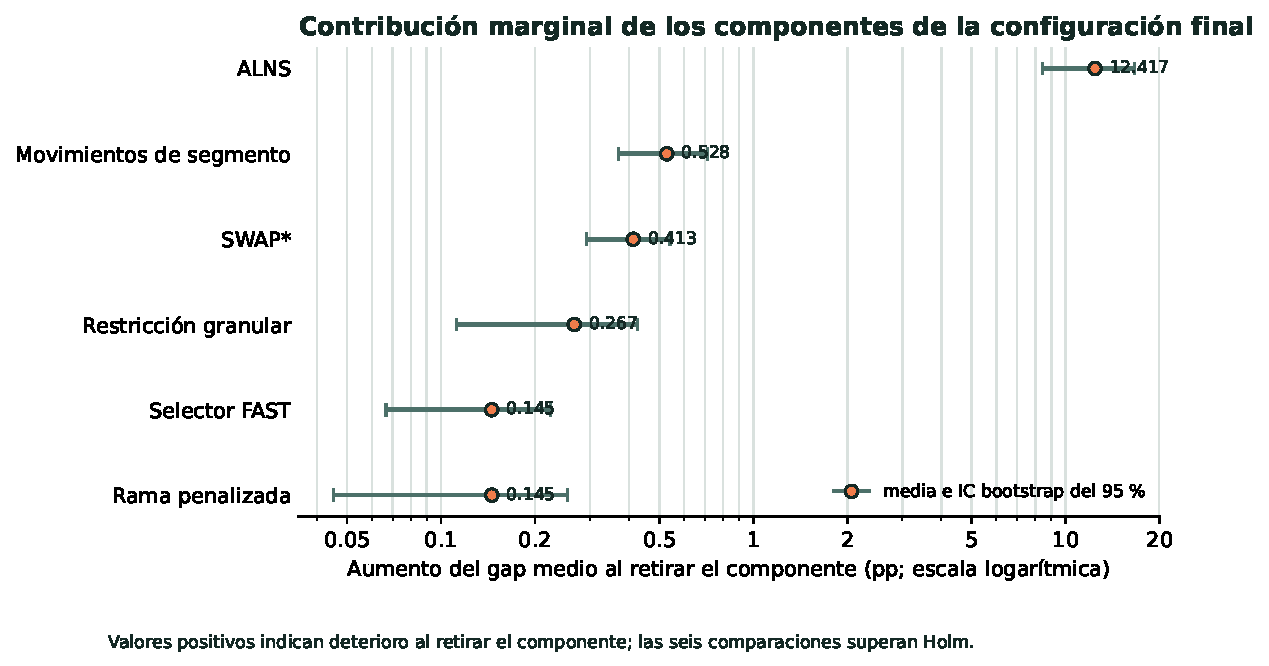
\includegraphics[width=0.82\linewidth]{figuras/F5_component_ablation_forest.pdf}
\caption{Aumento del gap al retirar cada componente (escala logarítmica). Todos los intervalos
bootstrap del 95\,\% quedan por encima de cero.}
\label{fig:forest}
\end{figure}

\begin{ideaclave}[: jerarquía de mecanismos]
El ALNS es el motor: sin él, el gap se multiplica por cuatro. Los movimientos entre rutas (segmentos
y SWAP*) forman un segundo nivel. El selector y el brazo penalizado son refinamientos de menor
magnitud.
\end{ideaclave}

\subsection{Holdout prospectivo}
El selector y sus umbrales se congelaron, con su huella SHA-256, antes de ejecutar 10 instancias X
que nunca se habían observado (\tsl{X-n351-k40} a \tsl{X-n429-k61}). En ellas los gaps medios
fueron 4.799\,\% para SENDA, 1.998\,\% para HGS y 0.740\,\% para FILO2. El orden entre métodos se
conserva: el selector funciona como regla fuera de las instancias de diseño, pero no convierte a SENDA
en el mejor solver de X.

% =========================================================================
\section{Caso de estudio: una auditoría que corrigió nuestros propios resultados}
\label{sec:caso}

\subsection{Qué se publicó}
La versión 2 reportaba en A/B/E un gap de 0.0120\,\% para SENDA frente a 0.0059\,\% para HGS, con 3
instancias ganadas por SENDA, 33 empates y 25 derrotas.

\subsection{Cómo se detectó el problema}
Al repetir la comparación en una campaña posterior aparecieron
\emph{gaps negativos}: soluciones de SENDA aparentemente mejores que el óptimo. Siguiendo la alarma de
la Sección~\ref{sec:cvrp}, se contaron las rutas de esas soluciones.

\begin{table}[H]
\centering
\caption{Soluciones con costo inferior a la BKS en los datos del proyecto. Ninguna es un récord
legítimo.}
\label{tab:bks}
\small
\begin{tabular}{@{}llrrl@{}}
\toprule
Instancia & BKS ($k$) & Solución & Rutas & Veredicto \\
\midrule
\tsl{B-n51-k7} & 1032 (7) & 1016 & 8 & usa un vehículo de más \\
\tsl{B-n57-k7} & 1153 (7) & 1140 & 8 & usa un vehículo de más \\
\tsl{E-n30-k3} & 534 (3) & 503 & 4 & usa un vehículo de más \\
\tsl{X-n247-k50}, \tsl{X-n420-k130} & --- & --- & --- & inválidas, ya excluidas en v2 \\
\bottomrule
\end{tabular}
\end{table}

\subsection{La causa}
El programa que lanzaba SENDA en los experimentos (el \emph{runner}) le indicaba ``flota libre'' incluso
en A/B/E, y su verificación comprobaba la cobertura y la capacidad, pero no el número de rutas. HGS,
en cambio, se ejecutó con la flota fija, y a FILO2 sí se le verificó la flota. En total, 327 corridas
de SENDA con más de $k$ rutas se aceptaron como válidas. Una revisión posterior de toda la carpeta del
proyecto mostró que el mismo problema afecta a los perfiles de sensibilidad de A/B/E (CPU igualada y
portafolio paralelo), cuyos gaps medios de SENDA también son negativos, y a la versión 1 del protocolo.

\subsection{La corrección}
\begin{enumerate}[leftmargin=1.5em]
\item Se repitió el análisis publicado a partir de los datos crudos y se obtuvo, byte a byte, la
misma tabla de comparaciones. Así se confirmó que el reanálisis no introducía cambios propios.
\item Se aplicó la misma regla de flota a todos los métodos. En los datos originales, tres
instancias se quedan sin ninguna réplica válida de SENDA, así que esos datos ya no sostienen la
comparación.
\item Se repitió el experimento con el runner corregido (flota igual a $k$), el mismo presupuesto,
las mismas semillas y HGS en el mismo bloque. Con la flota indicada, SENDA la respetó en las 630
corridas: el vehículo extra venía del runner, no del algoritmo. Ese es el resultado de la
Tabla~\ref{tab:abe}.
\end{enumerate}

\begin{leccion}[: verificar igual a todos]
Una comparación solo es justa si \emph{todos} los métodos se verifican con la misma regla. Aquí, una
diferencia de trato ---flota fija para HGS, flota libre para SENDA--- convirtió tres soluciones
inválidas en ``victorias''. Las señales de alarma existían: las familias B y E tenían gaps medios
negativos. Faltaba mirarlas con sospecha. La corrección mantiene la conclusión cualitativa (SENDA es
casi óptimo en A/B/E), pero cambia la magnitud de 0.012\,\% a 0.111\,\% y elimina toda victoria de
SENDA.
\end{leccion}

\begin{reproducir}
Datos originales: CSV canónico \tsl{f3a1164c85f4\ldots}. Re-corrida con flota fija y verificada:
contrato \tsl{fef9dd7ee521\ldots}. Para repetir la verificación con sus propios resultados, compruebe
en cada solución el número de rutas contra la flota de la instancia, además de la capacidad y la
cobertura (Sección~\ref{sec:pruebalo}).
\end{reproducir}

% =========================================================================
\section{Discusión}
\label{sec:discusion}

\paragraph{Dos regímenes.} En instancias de hasta cien clientes, \senda{} queda a una décima de punto
de la BKS en dos segundos; HGS es mejor, pero por poco. En instancias de 199 a 428 clientes, la
brecha frente a HGS y FILO2 crece a entre 2 y 3 puntos. La cascada sugiere por qué: en X, cada brazo
dispone de poco más de un segundo, y en ese tiempo su ALNS apenas mejora lo que ya logró la búsqueda
local (\cgfXd\,\% frente a \cgfXc\,\% en las soluciones factibles). El tiempo, no la construcción, es
el cuello de botella.

\paragraph{Significancia estadística frente a relevancia práctica.} Una diferencia de 0.1\,\% en
distancia puede ser irrelevante o importante según la operación. Cuando el ruteo se integra con
restricciones de carga tridimensional, ventanas de tiempo y reglas operativas, esas restricciones
suelen pesar más que las diferencias de ruteo puro. Cuantificarlo en el problema integrado es
trabajo futuro; este documento se limita al CVRP clásico.

\paragraph{Limitaciones.}
(i) La campaña principal y la re-corrida con flota fija se ejecutaron en máquinas distintas.
Dentro de cada comparación todos los métodos comparten máquina, pero no deben mezclarse cifras de
fuentes distintas.
(ii) El holdout contiene solo 10 instancias de una familia.
(iii) En X, la cascada usa el portafolio de A/B/E y no la variante X de la campaña principal
(4.150\,\% frente a 4.119\,\%).
(iv) La cascada se midió con el binario de la ablación, no con el confirmatorio.

% =========================================================================
\section{Conclusiones}
\label{sec:conclusiones}

\senda{} muestra que una arquitectura de trayectoria única por corrida, auditable y sin población alcanza una
calidad casi óptima en instancias clásicas pequeñas: 0.111\,\% de gap en 2\,s con la flota
verificada, aunque HGS es igual o mejor en todas ellas. En instancias X, HGS y FILO2 mantienen una
ventaja clara. La cascada y la ablación coinciden en que el ALNS es el mecanismo dominante, que los
movimientos entre rutas forman un segundo nivel y que el selector y el brazo penalizado afinan el
resultado.

Metodológicamente, el proyecto deja una enseñanza que vale más que cualquier cifra: la verificación
debe ser uniforme, los gaps negativos son alarmas y los resultados propios también deben auditarse.
Corregirlos públicamente no debilita el trabajo: lo hace creíble.

\paragraph{Trabajo futuro.}
(1) Dar más tiempo efectivo al ALNS en instancias grandes, por ejemplo evitando que cada brazo repita
la construcción y el pulido.
(2) Medir el impacto de estas diferencias en el problema integrado con carga tridimensional.
(3) Ampliar el holdout a otras familias y hasta $n=1000$.

\begin{reproducir}[: artefactos]
\small
\begin{tabular}{@{}p{4.9cm}p{9.6cm}@{}}
Campaña v2 (X, ablación, holdout) & contrato \tsl{36f29f1f1795\ldots}, CSV \tsl{f3a1164c85f4\ldots} \\
Corrección de flota & contrato \tsl{fef9dd7ee521\ldots} \\
Cascada de calidad & contrato \tsl{dd6b8817\ldots}; binario de ablación \tsl{4002751d\ldots} \\
Núcleo evaluado y HGS-CVRP & binario del núcleo \tsl{d7921fe1\ldots}; binario de HGS-CVRP \tsl{4e53fb18\ldots} \\
Figuras de este documento & datos en \tsl{paper/datos/} de este repositorio \\
Artefactos completos & archivo del autor; se comparten a solicitud (\tsl{contacto@lattimex.com}) \\
\end{tabular}
\end{reproducir}


% =========================================================================
\section{Pruébelo en su computadora}
\label{sec:pruebalo}

El motor de ruteo de LATTIMEX usa una versión posterior de SENDA (motor \tsl{1.6.0}): conserva sus componentes y agrega el portafolio en paralelo de la Sección~\ref{sec:portafolio}. Las cifras de esta guía se midieron con el binario \tsl{d7921fe1\ldots}, no con el del repositorio. El motor está publicado con licencia MIT en
\texttt{https://github.com/Erick-MF28/lattimex}. En el repositorio el núcleo es
\tsl{native/senda\_core.cpp}; alrededor de él hay una tubería que lo convierte en un planificador real:
capacidad efectiva, acomodo tridimensional de las cajas, mediación con flota fija y plan de descarga
por puertas. Los programas de comparación (HGS-CVRP, FILO2 y los scripts de las campañas) no forman
parte del repositorio.

\paragraph{1. Instalar y comprobar el motor.} Se necesita Python 3.10 o superior y un compilador de
C++ (en Windows basta \tsl{pip install ziglang}).
\begin{verbatim}
git clone https://github.com/Erick-MF28/lattimex.git
cd lattimex
pip install -r requirements.txt
python -m lattimex build        # compila el núcleo y el empacador 3D
python -m lattimex probe        # huella determinista (ver abajo)
python -m unittest discover -s tests/engine
\end{verbatim}
La huella determinista resume una corrida fija de 3\,000 iteraciones. Depende de la biblioteca
estándar de C++, porque \tsl{std::shuffle} y las distribuciones aleatorias se implementan distinto en
cada una: \tsl{6457b2dd44660773} con zig/libc++ (el instalador de Windows) y
\tsl{285bf1758e5dd6a1} con g++/libstdc++ (Linux y MinGW). Si su compilación da la huella de su
biblioteca, su binario calcula exactamente lo mismo que el publicado, aunque el archivo no sea
idéntico byte por byte.

\paragraph{2. Verlo trabajar sobre calles reales.} El motor construye su propio mapa a partir de
OpenStreetMap y lo sirve a la interfaz gráfica, el LATTIMEX Planner, que se abre en el navegador:
\begin{verbatim}
python -m lattimex map --bbox 20.47,-100.52,20.82,-100.22 --name queretaro
python -m lattimex serve        # luego abra https://lattimex.com/planner
\end{verbatim}
En la sección Guías del Planner, el botón \emph{Cargar ejemplo} agrega 300 entregas sintéticas en
Querétaro, seis vagonetas y cinco operarios; \emph{Optimizar} calcula las rutas y el acomodo de cada
caja. Los cálculos y los datos se quedan en su computadora.

\paragraph{3. Repetir una comparación de forma justa.} Para medir el núcleo en instancias de
referencia (CVRPLIB) contra otro solver, obtenga ese solver de su fuente oficial y respete las reglas
de la Sección~\ref{sec:evaluar}:
\begin{enumerate}[leftmargin=1.5em]
\item el mismo reloj de pared para todos los métodos, en la misma máquina y con un solo hilo;
\item al menos 10 réplicas con semillas distintas por instancia;
\item la misma flota para todos, fijada de antemano;
\item un verificador independiente que recalcule distancia, capacidad, cobertura y número de rutas;
\item comparaciones pareadas por instancia y corrección por comparaciones múltiples (Holm).
\end{enumerate}
Un gap negativo frente a la mejor solución conocida es, casi siempre, una alarma: revise primero la
flota y el redondeo de distancias.

\begin{ideaclave}
El código abierto permite que cualquiera repita las mediciones. Si sus resultados difieren de los de
esta guía, escríbanos: una discrepancia bien documentada es una contribución.
\end{ideaclave}

\bibliographystyle{plain}
\bibliography{referencias}

% =========================================================================
\appendix
\section{Glosario}
\label{app:glosario}
\begin{description}[leftmargin=0pt,font=\bfseries]
\item[BKS] Mejor solución conocida de una instancia de referencia.
\item[Gap] Diferencia relativa entre el costo obtenido y la BKS (ecuación~\ref{eq:gap}).
\item[Óptimo local] Solución que ningún movimiento de un vecindario dado puede mejorar.
\item[Réplica] Ejecución independiente con otra semilla. Aquí se usan 10 por instancia.
\item[Brazo] Una búsqueda independiente dentro de un ensayo; el portafolio tiene dos o tres.
\item[Tiempo de pared] Tiempo real transcurrido, medido con un reloj; se distingue del tiempo de CPU.
\item[Construcción] Procedimiento que genera la primera solución completa.
\item[Búsqueda local] Aplicación repetida de cambios pequeños que mejoran la solución.
\item[Restricción granular] Limitar los movimientos a pares de clientes cercanos.
\item[ALNS] Búsqueda adaptativa de vecindarios grandes: destruye y repara partes de la solución con
operadores cuyos pesos aprenden.
\item[Recocido simulado] Regla que acepta soluciones peores con una probabilidad que disminuye con el
tiempo.
\item[Regret-2] Reparación que inserta primero al cliente que más perdería si se le deja para
después.
\item[SWAP*] Intercambio de dos clientes entre rutas, cada uno en su mejor posición de la otra ruta.
\item[Portafolio] Configuración de SENDA evaluada en A/B/E: rama base, rama FAST y brazo penalizado.
\item[Brazo penalizado] Búsqueda que tolera excesos de capacidad temporales a cambio de una
penalización.
\item[Contrato] Archivo congelado con código, parámetros, instancias y pruebas, identificado por su
huella SHA-256.
\item[Holdout] Conjunto de instancias reservado y no observado durante el diseño.
\item[Holm] Corrección para comparaciones múltiples que controla el error de la familia de pruebas.
\item[$O$ grande] Notación que describe cómo crece el número de operaciones de un algoritmo con el
tamaño de la entrada (Sección~
ef{sec:complejidad}).
\end{description}

\section{Regla literal del selector FAST}
\label{app:selector}

\begin{algorithm}[H]
\caption{Configuración adicional elegida por FAST a partir de $\phi(I)$}
\begin{algorithmic}[1]
\Require $n$, $k$, presión de carga $\ell$, CV de demanda $c_q$, CV radial $c_r$, concentración angular $\alpha$, densidad $\eta$
\If{$n<150$}
  \SiDevolver{$n\ge70$}{\tsl{granular\_k25}}
  \If{$60\le n<70$}
    \SiDevolver{$\eta\ge0.0085$ o $\alpha<0.35$}{\tsl{large\_destroy\_k25}}
    \SiDevolver{$\alpha\ge0.80$}{\tsl{long\_10k\_k25}}
    \SiDevolver{$k\ge10$}{\tsl{granular\_k40}}
    \SiDevolver{$c_q<0.50$}{\tsl{long\_10k\_k25}}
    \State \Return \tsl{baseline}
  \EndIf
  \SiDevolver{$45\le n\le65$ y $\ell<0.93$ y $c_q<0.50$}{\tsl{medium\_destroy\_k25}}
  \State \Return \tsl{baseline}
\EndIf
\SiDevolver{$c_q\ge0.50$ y ($n\le245$ o $k\ge70$)}{\tsl{large\_destroy\_k25}}
\SiDevolver{$k\le16$ y [($c_q<0.30$ y $c_r<0.38$) o ($c_q<0.70$ y $\alpha\ge0.88$)]}{\tsl{granular\_k25}}
\SiDevolver{$k\ge55$ y $c_q\ge0.45$ y $\alpha\ge0.90$}{\tsl{granular\_k25}}
\SiDevolver{$n\ge300$ y $c_q\ge1.0$}{\tsl{baseline}}
\State \Return \tsl{long\_10k\_k25}
\end{algorithmic}
\end{algorithm}

\noindent Si la configuración elegida es \tsl{baseline}, el ensayo ejecuta solo la rama base y su
brazo penalizado. En otro caso ejecuta la rama base, la rama elegida y el brazo penalizado de esta
última.

\section{Errata respecto a la versión 2}
\label{app:errata}
\begin{itemize}[leftmargin=1.5em]
\item \textbf{A/B/E}: ``SENDA 0.0120\,\% frente a HGS 0.0059\,\%, 3/33/25, $p=0.00406$'' se sustituye
por ``SENDA 0.111\,\% frente a HGS 0.004\,\%, 0/37/23, $p=2.4\times10^{-7}$ (60 pares, flota fija
verificada)''.
\item \textbf{Verificación}: la afirmación de que se verificó la flota de cada solución no era cierta
para SENDA en la campaña v2; se corrigió en la re-corrida.
\item \textbf{Gates}: con la flota verificada, el gate de la comparación A/B/E de la campaña v2 falla;
los de X, ablación y holdout pasan sin cambios.
\item \textbf{Figura del mapa por instancia}: las tres celdas favorables a SENDA correspondían a
soluciones con $k+1$ vehículos (Figura~\ref{fig:abe}).
\end{itemize}

\end{document}
